% Options for packages loaded elsewhere
% Options for packages loaded elsewhere
\PassOptionsToPackage{unicode}{hyperref}
\PassOptionsToPackage{hyphens}{url}
\PassOptionsToPackage{dvipsnames,svgnames,x11names}{xcolor}
%
\documentclass[
  letterpaper,
  DIV=11,
  numbers=noendperiod]{scrreprt}
\usepackage{xcolor}
\usepackage{amsmath,amssymb}
\setcounter{secnumdepth}{5}
\usepackage{iftex}
\ifPDFTeX
  \usepackage[T1]{fontenc}
  \usepackage[utf8]{inputenc}
  \usepackage{textcomp} % provide euro and other symbols
\else % if luatex or xetex
  \usepackage{unicode-math} % this also loads fontspec
  \defaultfontfeatures{Scale=MatchLowercase}
  \defaultfontfeatures[\rmfamily]{Ligatures=TeX,Scale=1}
\fi
\usepackage{lmodern}
\ifPDFTeX\else
  % xetex/luatex font selection
\fi
% Use upquote if available, for straight quotes in verbatim environments
\IfFileExists{upquote.sty}{\usepackage{upquote}}{}
\IfFileExists{microtype.sty}{% use microtype if available
  \usepackage[]{microtype}
  \UseMicrotypeSet[protrusion]{basicmath} % disable protrusion for tt fonts
}{}
\makeatletter
\@ifundefined{KOMAClassName}{% if non-KOMA class
  \IfFileExists{parskip.sty}{%
    \usepackage{parskip}
  }{% else
    \setlength{\parindent}{0pt}
    \setlength{\parskip}{6pt plus 2pt minus 1pt}}
}{% if KOMA class
  \KOMAoptions{parskip=half}}
\makeatother
% Make \paragraph and \subparagraph free-standing
\makeatletter
\ifx\paragraph\undefined\else
  \let\oldparagraph\paragraph
  \renewcommand{\paragraph}{
    \@ifstar
      \xxxParagraphStar
      \xxxParagraphNoStar
  }
  \newcommand{\xxxParagraphStar}[1]{\oldparagraph*{#1}\mbox{}}
  \newcommand{\xxxParagraphNoStar}[1]{\oldparagraph{#1}\mbox{}}
\fi
\ifx\subparagraph\undefined\else
  \let\oldsubparagraph\subparagraph
  \renewcommand{\subparagraph}{
    \@ifstar
      \xxxSubParagraphStar
      \xxxSubParagraphNoStar
  }
  \newcommand{\xxxSubParagraphStar}[1]{\oldsubparagraph*{#1}\mbox{}}
  \newcommand{\xxxSubParagraphNoStar}[1]{\oldsubparagraph{#1}\mbox{}}
\fi
\makeatother

\usepackage{color}
\usepackage{fancyvrb}
\newcommand{\VerbBar}{|}
\newcommand{\VERB}{\Verb[commandchars=\\\{\}]}
\DefineVerbatimEnvironment{Highlighting}{Verbatim}{commandchars=\\\{\}}
% Add ',fontsize=\small' for more characters per line
\usepackage{framed}
\definecolor{shadecolor}{RGB}{241,243,245}
\newenvironment{Shaded}{\begin{snugshade}}{\end{snugshade}}
\newcommand{\AlertTok}[1]{\textcolor[rgb]{0.68,0.00,0.00}{#1}}
\newcommand{\AnnotationTok}[1]{\textcolor[rgb]{0.37,0.37,0.37}{#1}}
\newcommand{\AttributeTok}[1]{\textcolor[rgb]{0.40,0.45,0.13}{#1}}
\newcommand{\BaseNTok}[1]{\textcolor[rgb]{0.68,0.00,0.00}{#1}}
\newcommand{\BuiltInTok}[1]{\textcolor[rgb]{0.00,0.23,0.31}{#1}}
\newcommand{\CharTok}[1]{\textcolor[rgb]{0.13,0.47,0.30}{#1}}
\newcommand{\CommentTok}[1]{\textcolor[rgb]{0.37,0.37,0.37}{#1}}
\newcommand{\CommentVarTok}[1]{\textcolor[rgb]{0.37,0.37,0.37}{\textit{#1}}}
\newcommand{\ConstantTok}[1]{\textcolor[rgb]{0.56,0.35,0.01}{#1}}
\newcommand{\ControlFlowTok}[1]{\textcolor[rgb]{0.00,0.23,0.31}{\textbf{#1}}}
\newcommand{\DataTypeTok}[1]{\textcolor[rgb]{0.68,0.00,0.00}{#1}}
\newcommand{\DecValTok}[1]{\textcolor[rgb]{0.68,0.00,0.00}{#1}}
\newcommand{\DocumentationTok}[1]{\textcolor[rgb]{0.37,0.37,0.37}{\textit{#1}}}
\newcommand{\ErrorTok}[1]{\textcolor[rgb]{0.68,0.00,0.00}{#1}}
\newcommand{\ExtensionTok}[1]{\textcolor[rgb]{0.00,0.23,0.31}{#1}}
\newcommand{\FloatTok}[1]{\textcolor[rgb]{0.68,0.00,0.00}{#1}}
\newcommand{\FunctionTok}[1]{\textcolor[rgb]{0.28,0.35,0.67}{#1}}
\newcommand{\ImportTok}[1]{\textcolor[rgb]{0.00,0.46,0.62}{#1}}
\newcommand{\InformationTok}[1]{\textcolor[rgb]{0.37,0.37,0.37}{#1}}
\newcommand{\KeywordTok}[1]{\textcolor[rgb]{0.00,0.23,0.31}{\textbf{#1}}}
\newcommand{\NormalTok}[1]{\textcolor[rgb]{0.00,0.23,0.31}{#1}}
\newcommand{\OperatorTok}[1]{\textcolor[rgb]{0.37,0.37,0.37}{#1}}
\newcommand{\OtherTok}[1]{\textcolor[rgb]{0.00,0.23,0.31}{#1}}
\newcommand{\PreprocessorTok}[1]{\textcolor[rgb]{0.68,0.00,0.00}{#1}}
\newcommand{\RegionMarkerTok}[1]{\textcolor[rgb]{0.00,0.23,0.31}{#1}}
\newcommand{\SpecialCharTok}[1]{\textcolor[rgb]{0.37,0.37,0.37}{#1}}
\newcommand{\SpecialStringTok}[1]{\textcolor[rgb]{0.13,0.47,0.30}{#1}}
\newcommand{\StringTok}[1]{\textcolor[rgb]{0.13,0.47,0.30}{#1}}
\newcommand{\VariableTok}[1]{\textcolor[rgb]{0.07,0.07,0.07}{#1}}
\newcommand{\VerbatimStringTok}[1]{\textcolor[rgb]{0.13,0.47,0.30}{#1}}
\newcommand{\WarningTok}[1]{\textcolor[rgb]{0.37,0.37,0.37}{\textit{#1}}}

\usepackage{longtable,booktabs,array}
\usepackage{calc} % for calculating minipage widths
% Correct order of tables after \paragraph or \subparagraph
\usepackage{etoolbox}
\makeatletter
\patchcmd\longtable{\par}{\if@noskipsec\mbox{}\fi\par}{}{}
\makeatother
% Allow footnotes in longtable head/foot
\IfFileExists{footnotehyper.sty}{\usepackage{footnotehyper}}{\usepackage{footnote}}
\makesavenoteenv{longtable}
\usepackage{graphicx}
\makeatletter
\newsavebox\pandoc@box
\newcommand*\pandocbounded[1]{% scales image to fit in text height/width
  \sbox\pandoc@box{#1}%
  \Gscale@div\@tempa{\textheight}{\dimexpr\ht\pandoc@box+\dp\pandoc@box\relax}%
  \Gscale@div\@tempb{\linewidth}{\wd\pandoc@box}%
  \ifdim\@tempb\p@<\@tempa\p@\let\@tempa\@tempb\fi% select the smaller of both
  \ifdim\@tempa\p@<\p@\scalebox{\@tempa}{\usebox\pandoc@box}%
  \else\usebox{\pandoc@box}%
  \fi%
}
% Set default figure placement to htbp
\def\fps@figure{htbp}
\makeatother





\setlength{\emergencystretch}{3em} % prevent overfull lines

\providecommand{\tightlist}{%
  \setlength{\itemsep}{0pt}\setlength{\parskip}{0pt}}



 


\KOMAoption{captions}{tableheading}
\makeatletter
\@ifpackageloaded{bookmark}{}{\usepackage{bookmark}}
\makeatother
\makeatletter
\@ifpackageloaded{caption}{}{\usepackage{caption}}
\AtBeginDocument{%
\ifdefined\contentsname
  \renewcommand*\contentsname{Table of contents}
\else
  \newcommand\contentsname{Table of contents}
\fi
\ifdefined\listfigurename
  \renewcommand*\listfigurename{List of Figures}
\else
  \newcommand\listfigurename{List of Figures}
\fi
\ifdefined\listtablename
  \renewcommand*\listtablename{List of Tables}
\else
  \newcommand\listtablename{List of Tables}
\fi
\ifdefined\figurename
  \renewcommand*\figurename{Figure}
\else
  \newcommand\figurename{Figure}
\fi
\ifdefined\tablename
  \renewcommand*\tablename{Table}
\else
  \newcommand\tablename{Table}
\fi
}
\@ifpackageloaded{float}{}{\usepackage{float}}
\floatstyle{ruled}
\@ifundefined{c@chapter}{\newfloat{codelisting}{h}{lop}}{\newfloat{codelisting}{h}{lop}[chapter]}
\floatname{codelisting}{Listing}
\newcommand*\listoflistings{\listof{codelisting}{List of Listings}}
\makeatother
\makeatletter
\makeatother
\makeatletter
\@ifpackageloaded{caption}{}{\usepackage{caption}}
\@ifpackageloaded{subcaption}{}{\usepackage{subcaption}}
\makeatother
\usepackage{bookmark}
\IfFileExists{xurl.sty}{\usepackage{xurl}}{} % add URL line breaks if available
\urlstyle{same}
\hypersetup{
  pdftitle={Cambridge Supervisions},
  pdfauthor={Camilo Calderon},
  colorlinks=true,
  linkcolor={blue},
  filecolor={Maroon},
  citecolor={Blue},
  urlcolor={Blue},
  pdfcreator={LaTeX via pandoc}}


\title{Cambridge Supervisions}
\author{Camilo Calderon}
\date{}
\begin{document}
\maketitle

\renewcommand*\contentsname{Table of contents}
{
\hypersetup{linkcolor=}
\setcounter{tocdepth}{2}
\tableofcontents
}

\bookmarksetup{startatroot}

\chapter{Cambridge Supervisions}\label{cambridge-supervisions}

\bookmarksetup{startatroot}

\chapter{Welcome}\label{welcome}

This site hosts the supervision material for RM01 at the University of
Cambridge.\\
Use the sidebar to navigate to each lab.

\bookmarksetup{startatroot}

\chapter{Supervision 1}\label{supervision-1}

\section{\# Lab 1 --- R Certification (LinkedIn
Learning)}\label{lab-1-r-certification-linkedin-learning}

\section{Learning outcomes}\label{learning-outcomes}

By the end of this lab you will be able to: 1. Access \textbf{LinkedIn
Learning} via the University's UIS portal and sign in with SSO. 2.
Select a \textbf{beginner‑level R course/learning path} that issues a
certificate of completion. 3. Complete the course and \textbf{export
your certificate} (PDF/share link). 4. Add the certificate to your
\textbf{CV/LinkedIn profile}. 5. Run a short \textbf{tech‑check in
RStudio} to prepare for Labs 2--4.

\begin{center}\rule{0.5\linewidth}{0.5pt}\end{center}

\section{Prerequisites}\label{prerequisites}

\begin{itemize}
\tightlist
\item
  University credentials for LinkedIn Learning access.\\
\item
  R and RStudio installed (you'll run a small code check).\\
\item
  Stable internet connection.
\end{itemize}

\begin{center}\rule{0.5\linewidth}{0.5pt}\end{center}

\section{Part A --- First‑time access to LinkedIn
Learning}\label{part-a-firsttime-access-to-linkedin-learning}

\begin{enumerate}
\def\labelenumi{\arabic{enumi}.}
\tightlist
\item
  Follow the UIS guidance:
  \textbf{help.uis.cam.ac.uk/service/support/training/linkedin-learning-info}
  (opens the official instructions).\\
\item
  Choose \textbf{Sign in} with your University account (SSO). If
  prompted, connect to an existing LinkedIn profile (optional, but
  helpful for saving certificates).
\end{enumerate}

\textbf{Reflect:} What are the benefits/risks of linking your personal
LinkedIn account to the institutional LinkedIn Learning access?

\begin{center}\rule{0.5\linewidth}{0.5pt}\end{center}

\section{Part B --- Choose a beginner R
certificate}\label{part-b-choose-a-beginner-r-certificate}

\begin{enumerate}
\def\labelenumi{\arabic{enumi}.}
\tightlist
\item
  In LinkedIn Learning, search for \textbf{``R Programming''} or
  \textbf{``R for Data Analysis''}.\\
\item
  Pick a \textbf{Beginner} course or a \textbf{Learning Path} that
  issues a certificate upon completion.\\
\item
  Skim the syllabus; confirm it covers: R basics (objects, vectors),
  data frames, importing data, and simple plots.
\end{enumerate}

\textbf{Tip:} Short beginner certificates often take only a few hours.
Pick one you can finish this week.

\textbf{Reflect:} Which topics in your chosen course align best with
Planning, Growth \& Regeneration (e.g., data import, plotting
socio‑economic indicators)?

\begin{center}\rule{0.5\linewidth}{0.5pt}\end{center}

\section{Part C --- Complete the course
effectively}\label{part-c-complete-the-course-effectively}

\begin{itemize}
\tightlist
\item
  Turn on \textbf{captions} and adjust playback speed for focus.\\
\item
  Download \textbf{exercise files} (if offered) and practice in
  RStudio.\\
\item
  Take brief notes; collect 3--5 commands you didn't know before.\\
\item
  Mark lessons \textbf{Complete} as you go; attempt embedded quizzes.
\end{itemize}

\textbf{Reflect:} List three new R commands you learned and one common
error you corrected.

\begin{center}\rule{0.5\linewidth}{0.5pt}\end{center}

\section{Part D --- Export and submit your
certificate}\label{part-d-export-and-submit-your-certificate}

\begin{enumerate}
\def\labelenumi{\arabic{enumi}.}
\tightlist
\item
  After finishing, open the course page → \textbf{Certificate} →
  \textbf{Download PDF} (or \textbf{Copy share link}).\\
\item
  Save as \texttt{data/yourname\_r\_certificate.pdf}.\\
\item
  Submit the PDF to the LMS (or share link as instructed in your
  module).
\end{enumerate}

\textbf{Reflect:} Where will you showcase this credential (CV, LinkedIn,
portfolio)? Why?

\begin{center}\rule{0.5\linewidth}{0.5pt}\end{center}

\section{Part E --- Add to your LinkedIn profile (optional but
recommended)}\label{part-e-add-to-your-linkedin-profile-optional-but-recommended}

\begin{enumerate}
\def\labelenumi{\arabic{enumi}.}
\tightlist
\item
  Open your LinkedIn profile → \textbf{Add profile section} →
  \textbf{Recommended} → \textbf{Licenses \& Certifications}.\\
\item
  \textbf{Name:} Course title. \textbf{Issuing organization:} LinkedIn
  Learning. \textbf{Credential URL:} paste the certificate share link
  (if available).\\
\item
  Save.
\end{enumerate}

\textbf{Reflect:} How might this certification support applications for
placements or research roles in Land Economy?

\begin{center}\rule{0.5\linewidth}{0.5pt}\end{center}

\section{Part F --- RStudio tech‑check for upcoming
labs}\label{part-f-rstudio-techcheck-for-upcoming-labs}

Run these in RStudio to ensure you're ready for Labs 2--4.

\begin{Shaded}
\begin{Highlighting}[]
\NormalTok{R.version.string}
\end{Highlighting}
\end{Shaded}

\begin{verbatim}
[1] "R version 4.4.2 (2024-10-31 ucrt)"
\end{verbatim}

\begin{Shaded}
\begin{Highlighting}[]
\FunctionTok{sessionInfo}\NormalTok{()}\SpecialCharTok{$}\NormalTok{running}
\end{Highlighting}
\end{Shaded}

\begin{verbatim}
[1] "Windows 10 x64 (build 19045)"
\end{verbatim}

Install key packages (run once):

\begin{Shaded}
\begin{Highlighting}[]
\FunctionTok{install.packages}\NormalTok{(}\FunctionTok{c}\NormalTok{(}\StringTok{"learnr"}\NormalTok{, }\StringTok{"r4ds.tutorials"}\NormalTok{, }\StringTok{"readr"}\NormalTok{, }\StringTok{"readxl"}\NormalTok{, }\StringTok{"ggplot2"}\NormalTok{))}
\end{Highlighting}
\end{Shaded}

Verify they load and basic plotting works:

\begin{Shaded}
\begin{Highlighting}[]
\FunctionTok{library}\NormalTok{(ggplot2)}
\end{Highlighting}
\end{Shaded}

\begin{verbatim}
Warning: package 'ggplot2' was built under R version 4.4.3
\end{verbatim}

\begin{Shaded}
\begin{Highlighting}[]
\NormalTok{df }\OtherTok{\textless{}{-}} \FunctionTok{data.frame}\NormalTok{(}\AttributeTok{x =} \DecValTok{1}\SpecialCharTok{:}\DecValTok{10}\NormalTok{, }\AttributeTok{y =}\NormalTok{ (}\DecValTok{1}\SpecialCharTok{:}\DecValTok{10}\NormalTok{)}\SpecialCharTok{\^{}}\FloatTok{0.5}\NormalTok{)}
\FunctionTok{plot}\NormalTok{(df}\SpecialCharTok{$}\NormalTok{x, df}\SpecialCharTok{$}\NormalTok{y, }\AttributeTok{type =} \StringTok{"l"}\NormalTok{, }\AttributeTok{main =} \StringTok{"Tech‑check: base plot"}\NormalTok{, }\AttributeTok{xlab =} \StringTok{"x"}\NormalTok{, }\AttributeTok{ylab =} \StringTok{"sqrt(x)"}\NormalTok{)}
\end{Highlighting}
\end{Shaded}

\pandocbounded{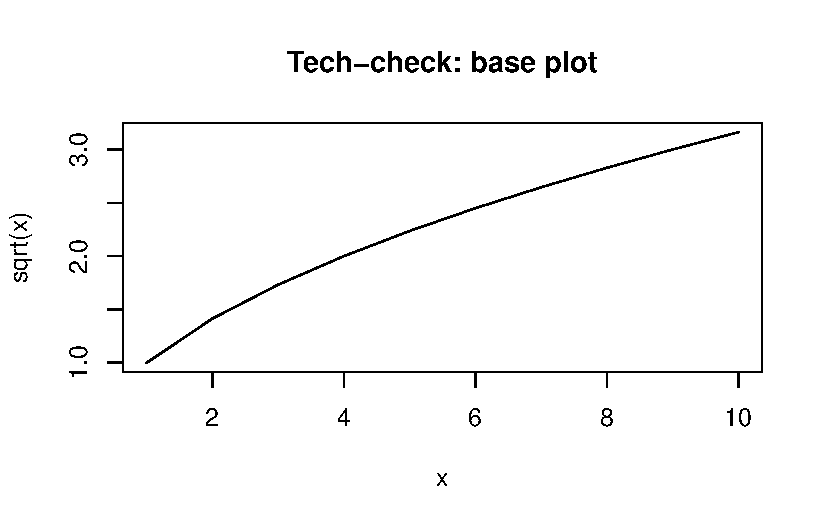
\includegraphics[keepaspectratio]{supervision_1_files/figure-pdf/unnamed-chunk-3-1.pdf}}

\textbf{Reflect:} Did everything install and run without warnings?
Capture any errors so we can fix them in class.

\begin{center}\rule{0.5\linewidth}{0.5pt}\end{center}

\section{Best practices}\label{best-practices}

\begin{itemize}
\tightlist
\item
  \textbf{Use institutional access} so your progress and certificates
  are recognized and free to you.\\
\item
  \textbf{Timebox} study sessions (e.g., 30--45 min focus blocks).\\
\item
  \textbf{Practice while you watch}---replicate examples in RStudio,
  don't just watch videos.\\
\item
  Keep a \textbf{snippets} file (your personal cheat‑sheet) with
  commands you'll reuse in Labs 3--4.\\
\item
  Store all artifacts (notes, PDFs) in your course project folder for
  quick reference.
\end{itemize}

\begin{center}\rule{0.5\linewidth}{0.5pt}\end{center}

\section{Suggested Answers
(indicative)}\label{suggested-answers-indicative}

\begin{itemize}
\tightlist
\item
  \textbf{Part A:} Linking accounts preserves learning history and makes
  sharing easy; a potential risk is mixing personal and institutional
  data---use privacy settings and review permissions.\\
\item
  \textbf{Part B:} Data import and plotting directly support
  planning/regeneration tasks (e.g., reading ONS data, visualising
  indicators).\\
\item
  \textbf{Part C:} Example new commands: \texttt{readr::read\_csv()},
  \texttt{dplyr::mutate()}, \texttt{ggplot2::geom\_line()}; common
  error: forgetting to load a package with \texttt{library()}.\\
\item
  \textbf{Part D:} Showcase on CV and LinkedIn; it signals foundational
  competency in R.\\
\item
  \textbf{Part E:} Certifications can strengthen internship or RA
  applications by evidencing practical skills.\\
\item
  \textbf{Part F:} If installs fail, note the exact error message; we'll
  address proxies, permissions, or missing system libraries next lab.
\end{itemize}

\begin{center}\rule{0.5\linewidth}{0.5pt}\end{center}

\emph{End of Lab 1}

\bookmarksetup{startatroot}

\chapter{Lab 2 --- Interactive R Learning (r4ds.tutorials + learnr +
swirl)}\label{lab-2-interactive-r-learning-r4ds.tutorials-learnr-swirl}

\begin{center}\rule{0.5\linewidth}{0.5pt}\end{center}

\section{Learning outcomes}\label{learning-outcomes-1}

By the end of this lab you will be able to: 1. Launch and complete the
\textbf{r4ds.tutorials} lesson \textbf{01-data-visualization} in
RStudio. 2. Run a built‑in \textbf{learnr} tutorial
(\textbf{ex-data-basics}) and submit answers in an interactive pane. 3.
Use \textbf{swirl} from the Console (install a course, resume lessons,
check progress). 4. Compare the strengths of r4ds.learnr tutorials
vs.~swirl for your own study plan.

\begin{center}\rule{0.5\linewidth}{0.5pt}\end{center}

\section{Prerequisites}\label{prerequisites-1}

\begin{itemize}
\tightlist
\item
  R (≥ 4.1) and RStudio.
\item
  Packages (install once):
\end{itemize}

\begin{Shaded}
\begin{Highlighting}[]
\FunctionTok{install.packages}\NormalTok{(}\FunctionTok{c}\NormalTok{(}\StringTok{"learnr"}\NormalTok{, }\StringTok{"r4ds.tutorials"}\NormalTok{, }\StringTok{"swirl"}\NormalTok{))}
\end{Highlighting}
\end{Shaded}

\begin{quote}
Tip: If tutorials don't appear in RStudio's \textbf{Tutorial} tab after
installation, restart R.
\end{quote}

\begin{center}\rule{0.5\linewidth}{0.5pt}\end{center}

\section{\texorpdfstring{Part A --- r4ds.tutorials:
\emph{01-data-visualization}}{Part A --- r4ds.tutorials: 01-data-visualization}}\label{part-a-r4ds.tutorials-01-data-visualization}

This runs as an interactive tutorial in RStudio's \textbf{Tutorial}
pane.

\begin{Shaded}
\begin{Highlighting}[]
\CommentTok{\# Option 1: via code}
\NormalTok{learnr}\SpecialCharTok{::}\FunctionTok{run\_tutorial}\NormalTok{(}\StringTok{"01{-}data{-}visualization"}\NormalTok{, }\AttributeTok{package =} \StringTok{"r4ds.tutorials"}\NormalTok{)}

\CommentTok{\# Option 2: discover tutorials installed on your system}
\NormalTok{learnr}\SpecialCharTok{::}\FunctionTok{available\_tutorials}\NormalTok{(}\StringTok{"r4ds.tutorials"}\NormalTok{)}
\end{Highlighting}
\end{Shaded}

\textbf{Do this:} 1. Start and complete the tutorial. Use the \emph{Show
in New Window} icon if the pane is small. 2. When you reach the
\textbf{Submit} page, follow its instructions (we won't collect
submissions in this lab, just finish to the end).

\textbf{Reflect:} - What's the difference between \textbf{aesthetics}
(e.g., \texttt{aes(x,\ y,\ color)}) and \textbf{geoms} (e.g.,
\texttt{geom\_point()}, \texttt{geom\_line()})? - Name two plot
improvements you used (labels, theme, scales, facets).

\begin{center}\rule{0.5\linewidth}{0.5pt}\end{center}

\section{\texorpdfstring{Part B --- learnr:
\emph{ex-data-basics}}{Part B --- learnr: ex-data-basics}}\label{part-b-learnr-ex-data-basics}

This is a short core tutorial bundled with \textbf{learnr}.

\begin{Shaded}
\begin{Highlighting}[]
\NormalTok{learnr}\SpecialCharTok{::}\FunctionTok{run\_tutorial}\NormalTok{(}\StringTok{"ex{-}data{-}basics"}\NormalTok{, }\AttributeTok{package =} \StringTok{"learnr"}\NormalTok{)}
\end{Highlighting}
\end{Shaded}

\textbf{Do this:} 1. Complete all exercises; click \textbf{Run} and
\textbf{Submit Answer} for each. 2. If you get stuck, open the
\textbf{Hint} dropdowns.

\textbf{Reflect:} - Which data types/structures did you manipulate
(vectors, data frames)? - One mistake you made and how the tutorial
feedback helped you fix it.

\begin{center}\rule{0.5\linewidth}{0.5pt}\end{center}

\section{Part C --- swirl
(console‑based)}\label{part-c-swirl-consolebased}

\textbf{swirl} runs entirely in the Console and saves your progress.

\begin{Shaded}
\begin{Highlighting}[]
\CommentTok{\# Install/run swirl}
\FunctionTok{install.packages}\NormalTok{(}\StringTok{"swirl"}\NormalTok{)}
\FunctionTok{library}\NormalTok{(swirl)}

\CommentTok{\# Start swirl}
\FunctionTok{swirl}\NormalTok{()}
\CommentTok{\# (enter your name when prompted)}

\CommentTok{\# Install and start a course (first time only)}
\FunctionTok{install\_from\_swirl}\NormalTok{(}\StringTok{"R Programming"}\NormalTok{)   }\CommentTok{\# or "R\_Programming"}

\CommentTok{\# At any time, leave swirl with}
\CommentTok{\# bye()}

\CommentTok{\# Check progress later}
\NormalTok{swirl}\SpecialCharTok{::}\FunctionTok{progress}\NormalTok{()}
\end{Highlighting}
\end{Shaded}

\textbf{Do this:} - Install \textbf{R Programming} and complete the
first lesson. - Exit with \texttt{bye()} and verify progress with
\texttt{swirl::progress()}.

\textbf{Reflect:} - How does working in the Console (swirl) feel
compared with the GUI tutorials? - Which mode gave you clearer feedback
on wrong answers?

\begin{center}\rule{0.5\linewidth}{0.5pt}\end{center}

\section{Part D --- Mini practice (5--10
min)}\label{part-d-mini-practice-510-min}

Create a tiny vector and compute a statistic, then plot a quick line:

\begin{Shaded}
\begin{Highlighting}[]
\NormalTok{x }\OtherTok{\textless{}{-}} \DecValTok{1}\SpecialCharTok{:}\DecValTok{10}
\NormalTok{mean\_x }\OtherTok{\textless{}{-}} \FunctionTok{mean}\NormalTok{(x)}
\NormalTok{mean\_x}
\end{Highlighting}
\end{Shaded}

\begin{verbatim}
[1] 5.5
\end{verbatim}

\begin{Shaded}
\begin{Highlighting}[]
\FunctionTok{plot}\NormalTok{(x, }\AttributeTok{type =} \StringTok{"l"}\NormalTok{, }\AttributeTok{main =} \StringTok{"Quick line"}\NormalTok{, }\AttributeTok{ylab =} \StringTok{"x"}\NormalTok{)}
\FunctionTok{abline}\NormalTok{(}\AttributeTok{h =}\NormalTok{ mean\_x, }\AttributeTok{lty =} \DecValTok{2}\NormalTok{)}
\end{Highlighting}
\end{Shaded}

\pandocbounded{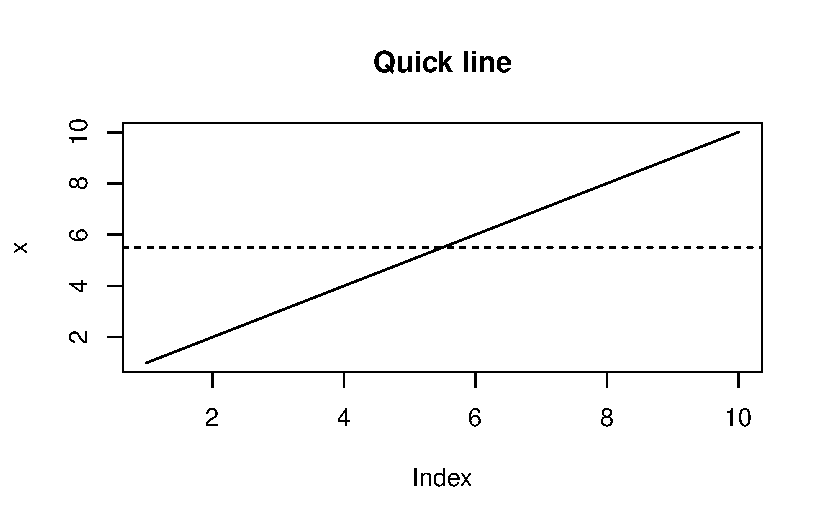
\includegraphics[keepaspectratio]{supervision_1_files/figure-pdf/unnamed-chunk-8-1.pdf}}

\textbf{Reflect:} - Which approach (r4ds.tutorials, learnr, swirl) best
prepared you to write and run this code independently?

\begin{center}\rule{0.5\linewidth}{0.5pt}\end{center}

\section{Best practices}\label{best-practices-1}

\begin{itemize}
\tightlist
\item
  \textbf{Use learnr/r4ds.tutorials for guided practice} with hints,
  auto‑checks, and saved state.
\item
  \textbf{Use swirl} when you prefer keyboard‑only Console practice or
  have limited UI.
\item
  Restart RStudio if tutorials don't show; list what's available with
  \texttt{learnr::available\_tutorials()}.
\item
  Keep your scripts open alongside tutorials to copy refined solutions
  into your own notes.
\end{itemize}

\begin{center}\rule{0.5\linewidth}{0.5pt}\end{center}

\section{Suggested Answers
(indicative)}\label{suggested-answers-indicative-1}

\begin{itemize}
\tightlist
\item
  \textbf{Part A:} Aesthetics map data → visual channels; geoms are the
  drawing layers (points, lines, bars). Improvements often include
  \texttt{labs()}, \texttt{scale\_*\_continuous()},
  \texttt{theme\_minimal()}, and \texttt{facet\_wrap()}.
\item
  \textbf{Part B:} Worked with vectors/data frames; common mistakes
  include mixing types (character vs numeric) or forgetting
  \texttt{\textless{}-}. Hints/feedback indicate expected objects or
  function names.
\item
  \textbf{Part C:} Console is lightweight but less visual; learnr/r4ds
  tutorials give more structured feedback. Swirl progress persists via
  \texttt{swirl::progress()}; exit with \texttt{bye()}.
\item
  \textbf{Part D:} Any of the three can help; most students report
  faster iteration in learnr/r4ds due to inline errors/hints.
\end{itemize}

\begin{center}\rule{0.5\linewidth}{0.5pt}\end{center}

\emph{End of Lab 2}

\bookmarksetup{startatroot}

\chapter{Lab 3 --- Uploading Excel \& CSV Files to R
(PIPR)}\label{lab-3-uploading-excel-csv-files-to-r-pipr}

\begin{center}\rule{0.5\linewidth}{0.5pt}\end{center}

\section{Learning outcomes}\label{learning-outcomes-2}

By the end of this lab you will be able to: 1. Download the \textbf{ONS
Price Index of Private Rents (PIPR)} monthly workbook and save it in a
tidy project structure. 2. Import \textbf{Excel} (\texttt{.xlsx/.xls})
and \textbf{CSV} files using RStudio's \textbf{Import Dataset} UI
\textbf{and} reproducible R code. 3. Deal with metadata/header rows via
\texttt{skip}, set \texttt{col\_names}, and verify column
\textbf{types}. 4. Plot time series (index and annual \% change) with
base R and add reference lines. 5. Use help pages (e.g., \texttt{?plot})
and annotate charts for a policy audience.

\begin{center}\rule{0.5\linewidth}{0.5pt}\end{center}

\section{Prerequisites}\label{prerequisites-2}

\begin{itemize}
\tightlist
\item
  R (≥ 4.0) and RStudio.
\item
  Project folder (e.g., \texttt{Rcoding/}) with subfolder
  \texttt{data/}.
\item
  Packages (install once):
\end{itemize}

\begin{Shaded}
\begin{Highlighting}[]
\CommentTok{\# install.packages(c("readxl", "readr"))}
\end{Highlighting}
\end{Shaded}

\begin{quote}
\textbf{Tip:} Prefer file names without spaces and lower-cases,
e.g.~\texttt{pipr\_monthly.xls} rather than \texttt{pipr\ monthly.xls}.
\end{quote}

\begin{center}\rule{0.5\linewidth}{0.5pt}\end{center}

\section{Part A --- Get PIPR monthly from ONS (manual
steps)}\label{part-a-get-pipr-monthly-from-ons-manual-steps}

\begin{enumerate}
\def\labelenumi{\arabic{enumi}.}
\item
  Go to \textbf{ONS.gov.uk} and search \textbf{Price Index of Private
  Rents (PIPR)}. This lab is using ONS data on Figure 4: Rent annual
  inflation slowed across the UK, Private rents annual inflation, across
  the UK, January 2016 to August 2025.
\item
  On the dataset page, choose \textbf{Data} → \textbf{Download monthly
  workbook} (Excel) or \textbf{CSV} if available.
\item
  Save as \texttt{data/pipr\_monthly.xls} inside your project folder
  (e.g., \texttt{Rcoding/}) with subfolder \texttt{data/}.
\item
  (Optional) Open the file and identify the sheet that contains the
  \textbf{UK} and \textbf{country/regions}.
\end{enumerate}

\textbf{Reflect:} Why does PIPR (rents) provide a more direct lens on
housing affordability and regional pressures than GDP for planning and
regeneration?

\begin{center}\rule{0.5\linewidth}{0.5pt}\end{center}

\section{Part B --- Import Excel via code
(reproducible)}\label{part-b-import-excel-via-code-reproducible}

Use \texttt{readxl::read\_excel()} and inspect column names to choose
the UK series.

\begin{Shaded}
\begin{Highlighting}[]
\FunctionTok{library}\NormalTok{(readxl)}
\CommentTok{\# Adjust \textquotesingle{}sheet\textquotesingle{} and \textquotesingle{}skip\textquotesingle{} depending on the workbook structure you download.}
\CommentTok{\# we use skip = 7 because there are headings in the first 7 rows of the dataset.}
\NormalTok{pipr\_raw }\OtherTok{\textless{}{-}} \FunctionTok{read\_excel}\NormalTok{(}\StringTok{"data/pipr\_monthly.xls"}\NormalTok{, }\AttributeTok{sheet =} \DecValTok{1}\NormalTok{, }\AttributeTok{skip =} \DecValTok{7}\NormalTok{)}

\CommentTok{\# Inspect names to locate the date/month, UK Index, and UK annual \% change columns}
\FunctionTok{names}\NormalTok{(pipr\_raw)}
\end{Highlighting}
\end{Shaded}

\begin{verbatim}
[1] "Date"             "UK"               "England"          "Wales"           
[5] "Scotland"         "Northern Ireland"
\end{verbatim}

\begin{Shaded}
\begin{Highlighting}[]
\CommentTok{\# let\textquotesingle{}s keep a copy of the raw data intact and create a new version of the data.}

\NormalTok{pipr}\OtherTok{\textless{}{-}}\NormalTok{pipr\_raw}

\CommentTok{\# rename column names for easiness. }
\FunctionTok{names}\NormalTok{(pipr) }\OtherTok{\textless{}{-}} \FunctionTok{c}\NormalTok{(}\StringTok{"month"}\NormalTok{, }\StringTok{"uk"}\NormalTok{, }\StringTok{"england"}\NormalTok{, }\StringTok{"wales"}\NormalTok{, }\StringTok{"scotland"}\NormalTok{, }\StringTok{"n\_ireland"}\NormalTok{)}

\FunctionTok{str}\NormalTok{(pipr)}
\end{Highlighting}
\end{Shaded}

\begin{verbatim}
tibble [116 x 6] (S3: tbl_df/tbl/data.frame)
 $ month    : POSIXct[1:116], format: "2016-01-01" "2016-02-01" ...
 $ uk       : num [1:116] 3.3 3.3 3.4 3.3 3.2 3.3 3.4 3.3 3.2 3.3 ...
 $ england  : num [1:116] 3.5 3.5 3.6 3.5 3.3 3.5 3.7 3.6 3.5 3.6 ...
 $ wales    : num [1:116] 1.2 0.8 0.8 0.6 0.4 0.3 0.3 0.9 1.4 1.3 ...
 $ scotland : num [1:116] 2.1 1.8 1.6 1.5 1.4 1.1 1.2 0.9 1.1 1.1 ...
 $ n_ireland: num [1:116] 1.1 1.3 1.4 1.6 1.6 1.6 1.5 1.5 1 0.9 ...
\end{verbatim}

\begin{Shaded}
\begin{Highlighting}[]
\FunctionTok{head}\NormalTok{(pipr, }\DecValTok{6}\NormalTok{)}
\end{Highlighting}
\end{Shaded}

\begin{verbatim}
# A tibble: 6 x 6
  month                  uk england wales scotland n_ireland
  <dttm>              <dbl>   <dbl> <dbl>    <dbl>     <dbl>
1 2016-01-01 00:00:00   3.3     3.5   1.2      2.1       1.1
2 2016-02-01 00:00:00   3.3     3.5   0.8      1.8       1.3
3 2016-03-01 00:00:00   3.4     3.6   0.8      1.6       1.4
4 2016-04-01 00:00:00   3.3     3.5   0.6      1.5       1.6
5 2016-05-01 00:00:00   3.2     3.3   0.4      1.4       1.6
6 2016-06-01 00:00:00   3.3     3.5   0.3      1.1       1.6
\end{verbatim}

\textbf{Reflect:} Are the three selected columns correct for your
workbook version? If not, which names should you use instead?

\begin{center}\rule{0.5\linewidth}{0.5pt}\end{center}

\section{Part C --- Import via RStudio UI
(reference)}\label{part-c-import-via-rstudio-ui-reference}

\begin{itemize}
\tightlist
\item
  RStudio → \textbf{Import Dataset} → \textbf{From Excel} → select
  \texttt{data/pipr\_monthly.xls}.
\item
  Choose the relevant \textbf{sheet} and, if needed, set \textbf{Skip}
  for metadata rows.
\item
  Set \textbf{Name} to \texttt{pipr} and verify column names (e.g.,
  \texttt{month}, \texttt{uk\_index}, \texttt{uk\_yoy}).
\item
  Click \textbf{Copy} to grab the generated R code, then
  \textbf{Import}.
\end{itemize}

\begin{quote}
Paste the generated code in your script so your workflow is
\textbf{reproducible}.
\end{quote}

\begin{center}\rule{0.5\linewidth}{0.5pt}\end{center}

\section{Part D --- Basic time‑series line plot (annual \%
change)}\label{part-d-basic-timeseries-line-plot-annual-change}

Plot PIPR annual \% change for the UK as a line. Label the x‑axis
sparsely to keep it readable.

\begin{Shaded}
\begin{Highlighting}[]
\FunctionTok{plot}\NormalTok{(pipr}\SpecialCharTok{$}\NormalTok{uk, }\AttributeTok{type =} \StringTok{"l"}\NormalTok{,}
     \AttributeTok{xlab =} \StringTok{""}\NormalTok{,}
     \AttributeTok{ylab =} \StringTok{"Private rents — annual \% change"}\NormalTok{,}
     \AttributeTok{main =} \StringTok{"UK private rents (PIPR): annual \% change"}\NormalTok{,}
     \AttributeTok{xaxt =} \StringTok{"n"}\NormalTok{)   }\CommentTok{\# suppress default axis)}

\CommentTok{\# Add sparse x{-}axis labels}
\NormalTok{labs\_every }\OtherTok{\textless{}{-}} \DecValTok{6}
\NormalTok{at\_idx }\OtherTok{\textless{}{-}} \FunctionTok{seq}\NormalTok{(}\DecValTok{1}\NormalTok{, }\FunctionTok{nrow}\NormalTok{(pipr), }\AttributeTok{by =}\NormalTok{ labs\_every)}
\FunctionTok{axis}\NormalTok{(}\DecValTok{1}\NormalTok{, }\AttributeTok{at =}\NormalTok{ at\_idx, }\AttributeTok{labels =}\NormalTok{ pipr}\SpecialCharTok{$}\NormalTok{month[at\_idx],}
     \AttributeTok{las =} \DecValTok{2}\NormalTok{, }\AttributeTok{cex.axis =} \FloatTok{0.7}\NormalTok{)  }\CommentTok{\# smaller font for ticks}

\CommentTok{\# Add subtitle (source) directly under the title}
\FunctionTok{title}\NormalTok{(}\AttributeTok{sub =} \StringTok{"Source: ONS {-} Index of Private Housing Rental Prices (PIPR)"}\NormalTok{, }
      \AttributeTok{cex.sub =} \FloatTok{0.8}\NormalTok{, }\AttributeTok{font.sub =} \DecValTok{3}\NormalTok{)  }\CommentTok{\# italic, smaller}
\CommentTok{\# Reference line at 2\% (inflation target)}
\FunctionTok{abline}\NormalTok{(}\AttributeTok{h =} \DecValTok{2}\NormalTok{, }\AttributeTok{lty =} \DecValTok{2}\NormalTok{, }\AttributeTok{col =} \StringTok{"blue"}\NormalTok{)}

\CommentTok{\# Label it}
\FunctionTok{text}\NormalTok{(}\AttributeTok{x =} \FunctionTok{min}\NormalTok{(pipr}\SpecialCharTok{$}\NormalTok{month), }\AttributeTok{y =} \DecValTok{2}\NormalTok{, }\AttributeTok{labels =} \StringTok{"Inflation target (2\%)"}\NormalTok{,}
     \AttributeTok{pos =} \DecValTok{3}\NormalTok{, }\AttributeTok{col =} \StringTok{"blue"}\NormalTok{, }\AttributeTok{cex =} \FloatTok{0.8}\NormalTok{)}
\end{Highlighting}
\end{Shaded}

\pandocbounded{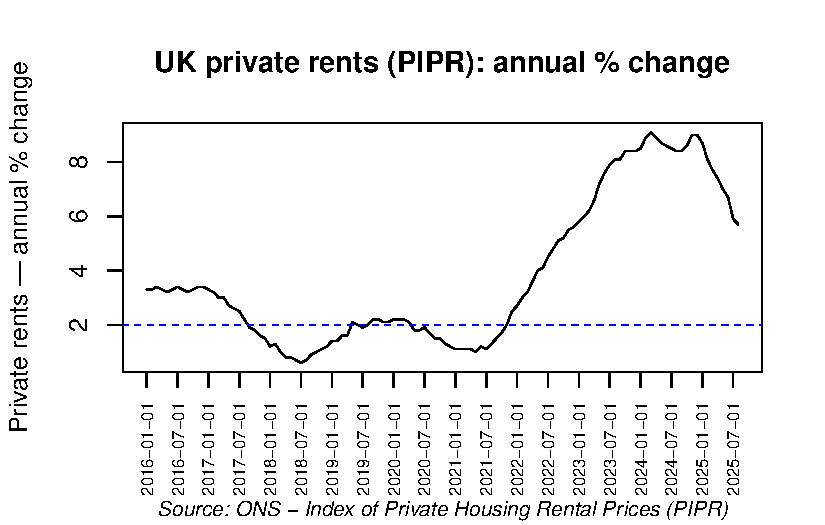
\includegraphics[keepaspectratio]{supervision_1_files/figure-pdf/unnamed-chunk-11-1.pdf}}

\textbf{Reflect:} Identify periods of fastest rent inflation and periods
of slowdown. What policy or macro factors might line up with these
shifts?

\begin{center}\rule{0.5\linewidth}{0.5pt}\end{center}

\section{Part E --- Blue reference line at 2\% (Inflation Target) \&
customise}\label{part-e-blue-reference-line-at-2-inflation-target-customise}

\textbf{Reflect:} What extra annotations (e.g., policy changes, shocks)
would make this plot more useful to a local authority audience?

\begin{center}\rule{0.5\linewidth}{0.5pt}\end{center}

\section{Part F --- Import PIPR as CSV
(alternative)}\label{part-f-import-pipr-as-csv-alternative}

Option 1: Download the \textbf{CSV} from the PIPR page (if provided) and
import with \texttt{readr::read\_csv()}.

\begin{Shaded}
\begin{Highlighting}[]
\FunctionTok{library}\NormalTok{(readr)}
\NormalTok{pipr\_csv }\OtherTok{\textless{}{-}} \FunctionTok{read\_csv}\NormalTok{(}\StringTok{"data/pipr\_monthly.csv"}\NormalTok{)  }\CommentTok{\# adjust file name}
\end{Highlighting}
\end{Shaded}

\begin{verbatim}
New names:
Rows: 130 Columns: 9
-- Column specification
-------------------------------------------------------- Delimiter: "," chr
(6): Figure 4: Rent annual inflation slowed across the UK, ...2, ...3, .... lgl
(3): ...7, ...8, ...9
i Use `spec()` to retrieve the full column specification for this data. i
Specify the column types or set `show_col_types = FALSE` to quiet this message.
* `` -> `...2`
* `` -> `...3`
* `` -> `...4`
* `` -> `...5`
* `` -> `...6`
* `` -> `...7`
* `` -> `...8`
* `` -> `...9`
\end{verbatim}

\begin{Shaded}
\begin{Highlighting}[]
\FunctionTok{names}\NormalTok{(pipr\_csv)}
\end{Highlighting}
\end{Shaded}

\begin{verbatim}
[1] "Figure 4: Rent annual inflation slowed across the UK"
[2] "...2"                                                
[3] "...3"                                                
[4] "...4"                                                
[5] "...5"                                                
[6] "...6"                                                
[7] "...7"                                                
[8] "...8"                                                
[9] "...9"                                                
\end{verbatim}

\begin{Shaded}
\begin{Highlighting}[]
\FunctionTok{head}\NormalTok{(pipr\_csv)}
\end{Highlighting}
\end{Shaded}

\begin{verbatim}
# A tibble: 6 x 9
  Figure 4: Rent annual inflat~1 ...2  ...3  ...4  ...5  ...6  ...7  ...8  ...9 
  <chr>                          <chr> <chr> <chr> <chr> <chr> <lgl> <lgl> <lgl>
1 Private rents annual inflatio~  <NA> <NA>  <NA>  <NA>  <NA>  NA    NA    NA   
2 <NA>                            <NA> <NA>  <NA>  <NA>  <NA>  NA    NA    NA   
3 Notes                          "1. ~ <NA>  <NA>  <NA>  <NA>  NA    NA    NA   
4 Unit                           "Per~ <NA>  <NA>  <NA>  <NA>  NA    NA    NA   
5 Source                         "Pri~ <NA>  <NA>  <NA>  <NA>  NA    NA    NA   
6 <NA>                            <NA> <NA>  <NA>  <NA>  <NA>  NA    NA    NA   
# i abbreviated name: 1: `Figure 4: Rent annual inflation slowed across the UK`
\end{verbatim}

Option 2: If a CSV isn't provided, \textbf{save the relevant sheet as
CSV} from Excel and import it.

\begin{Shaded}
\begin{Highlighting}[]
\CommentTok{\# Example: write out the subset you prepared, then re{-}import it}
\CommentTok{\# write\_csv(pipr, "data/pipr\_monthly\_subset.csv")}
\NormalTok{pipr\_from\_csv }\OtherTok{\textless{}{-}} \FunctionTok{read\_csv}\NormalTok{(}\StringTok{"data/pipr\_monthly.csv"}\NormalTok{)}
\end{Highlighting}
\end{Shaded}

\begin{verbatim}
New names:
Rows: 130 Columns: 9
-- Column specification
-------------------------------------------------------- Delimiter: "," chr
(6): Figure 4: Rent annual inflation slowed across the UK, ...2, ...3, .... lgl
(3): ...7, ...8, ...9
i Use `spec()` to retrieve the full column specification for this data. i
Specify the column types or set `show_col_types = FALSE` to quiet this message.
* `` -> `...2`
* `` -> `...3`
* `` -> `...4`
* `` -> `...5`
* `` -> `...6`
* `` -> `...7`
* `` -> `...8`
* `` -> `...9`
\end{verbatim}

\textbf{Reflect:} Are types preserved across Excel vs CSV imports? Which
route is more reliable/reproducible on your machine?

\begin{center}\rule{0.5\linewidth}{0.5pt}\end{center}

\section{Part G --- Compare UK with a region
(optional)}\label{part-g-compare-uk-with-a-region-optional}

If your workbook includes regions (England, Wales, Scotland, Northern
Ireland), select one annual \% change column and plot together with the
UK.

\begin{Shaded}
\begin{Highlighting}[]
\CommentTok{\# Attempt to find a regional YoY column (edit the pattern or use exact name after checking names())}
\NormalTok{reg\_yoy\_col }\OtherTok{\textless{}{-}} \FunctionTok{grep}\NormalTok{(}\StringTok{"England.*Annual|Annual.*England|England.*\%"}\NormalTok{, }\FunctionTok{names}\NormalTok{(pipr\_raw), }\AttributeTok{ignore.case =} \ConstantTok{TRUE}\NormalTok{)[}\DecValTok{1}\NormalTok{]}

\ControlFlowTok{if}\NormalTok{(}\SpecialCharTok{!}\FunctionTok{is.na}\NormalTok{(reg\_yoy\_col))\{}
\NormalTok{  reg\_yoy }\OtherTok{\textless{}{-}} \FunctionTok{suppressWarnings}\NormalTok{(}\FunctionTok{as.numeric}\NormalTok{(pipr\_raw[[reg\_yoy\_col]]))}
  \FunctionTok{plot}\NormalTok{(pipr}\SpecialCharTok{$}\NormalTok{uk\_yoy, }\AttributeTok{type =} \StringTok{"l"}\NormalTok{, }\AttributeTok{xlab =} \StringTok{"Month"}\NormalTok{, }\AttributeTok{ylab =} \StringTok{"Annual \% change"}\NormalTok{,}
       \AttributeTok{main =} \StringTok{"PIPR annual \% change: UK vs England"}\NormalTok{)}
  \FunctionTok{lines}\NormalTok{(reg\_yoy, }\AttributeTok{lty =} \DecValTok{3}\NormalTok{)}
  \FunctionTok{legend}\NormalTok{(}\StringTok{"topleft"}\NormalTok{, }\AttributeTok{legend =} \FunctionTok{c}\NormalTok{(}\StringTok{"UK"}\NormalTok{, }\StringTok{"England"}\NormalTok{), }\AttributeTok{lty =} \FunctionTok{c}\NormalTok{(}\DecValTok{1}\NormalTok{,}\DecValTok{3}\NormalTok{), }\AttributeTok{bty =} \StringTok{"n"}\NormalTok{)}
\NormalTok{\} }\ControlFlowTok{else}\NormalTok{ \{}
  \FunctionTok{message}\NormalTok{(}\StringTok{"No matching regional column automatically detected — inspect names() and set reg\_yoy\_col manually."}\NormalTok{)}
\NormalTok{\}}
\end{Highlighting}
\end{Shaded}

\begin{verbatim}
No matching regional column automatically detected — inspect names() and set reg_yoy_col manually.
\end{verbatim}

\textbf{Reflect:} Does the region move broadly with the UK or diverge
materially? What local factors could explain divergence?

\begin{center}\rule{0.5\linewidth}{0.5pt}\end{center}

\section{Part H --- Help pages and plotting
extras}\label{part-h-help-pages-and-plotting-extras}

Explore \texttt{?plot}, \texttt{curve()}, and \texttt{abline()}.

\begin{Shaded}
\begin{Highlighting}[]
\CommentTok{\# ?plot   \# open during interactive session}
\FunctionTok{curve}\NormalTok{(}\FunctionTok{sin}\NormalTok{(x), }\AttributeTok{from =} \DecValTok{0}\NormalTok{, }\AttributeTok{to =} \FloatTok{6.28}\NormalTok{, }\AttributeTok{xlab =} \StringTok{"x"}\NormalTok{, }\AttributeTok{ylab =} \StringTok{"y = sin(x)"}\NormalTok{)}
\end{Highlighting}
\end{Shaded}

\pandocbounded{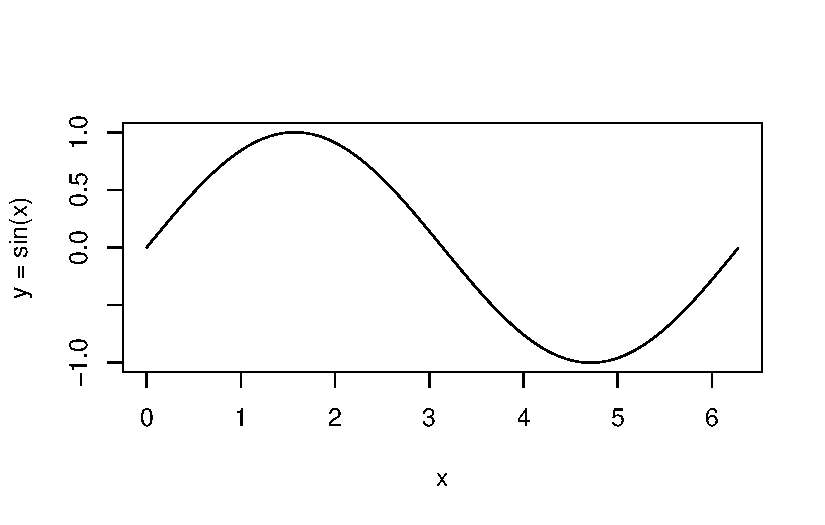
\includegraphics[keepaspectratio]{supervision_1_files/figure-pdf/unnamed-chunk-15-1.pdf}}

\begin{Shaded}
\begin{Highlighting}[]
\FunctionTok{plot}\NormalTok{(}\DecValTok{1}\SpecialCharTok{:}\DecValTok{10}\NormalTok{, }\AttributeTok{type =} \StringTok{"n"}\NormalTok{, }\AttributeTok{xlab =} \StringTok{"x"}\NormalTok{, }\AttributeTok{ylab =} \StringTok{"y"}\NormalTok{)}
\FunctionTok{abline}\NormalTok{(}\AttributeTok{h =} \DecValTok{0}\NormalTok{, }\AttributeTok{v =} \DecValTok{5}\NormalTok{, }\AttributeTok{lty =} \DecValTok{2}\NormalTok{)}
\end{Highlighting}
\end{Shaded}

\pandocbounded{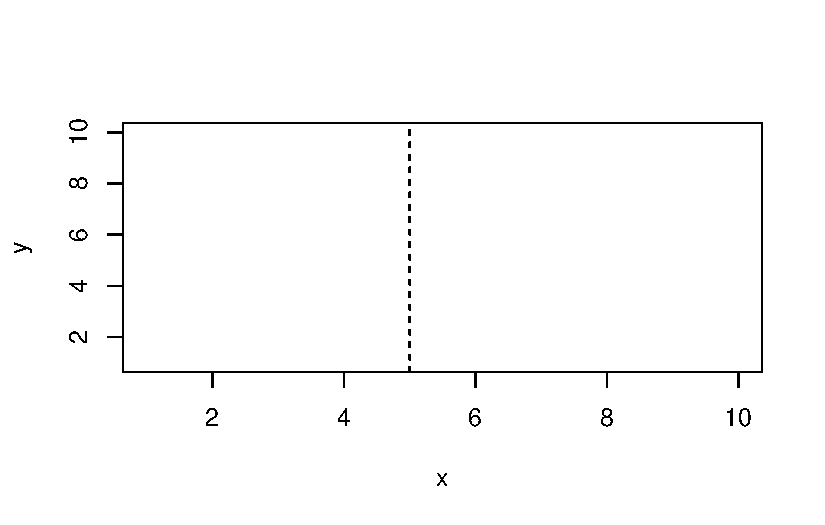
\includegraphics[keepaspectratio]{supervision_1_files/figure-pdf/unnamed-chunk-15-2.pdf}}

\textbf{Reflect:} Which \texttt{plot()} arguments improved readability
most (e.g., \texttt{las}, \texttt{xaxt}, \texttt{lwd}, \texttt{xlim})?

\begin{center}\rule{0.5\linewidth}{0.5pt}\end{center}

\section{Part I --- (Optional) Principles of Econometrics
data}\label{part-i-optional-principles-of-econometrics-data}

You can also explore textbook datasets with \textbf{PoEdata} for
practice with scatter plots and \texttt{abline(lm())}.

\begin{Shaded}
\begin{Highlighting}[]
\CommentTok{\#install.packages(c("remotes", "pkgbuild"))   \# helper packages}
\CommentTok{\#pkgbuild::has\_build\_tools(debug = TRUE)       \# should say TRUE on Windows}
\CommentTok{\#remotes::install\_github("ccolonescu/PoEdata")}
\FunctionTok{library}\NormalTok{(PoEdata)}

\FunctionTok{data}\NormalTok{(}\StringTok{"andy"}\NormalTok{)}
\FunctionTok{head}\NormalTok{(andy)}
\end{Highlighting}
\end{Shaded}

\begin{verbatim}
  sales price advert
1  73.2  5.69    1.3
2  71.8  6.49    2.9
3  62.4  5.63    0.8
4  67.4  6.22    0.7
5  89.3  5.02    1.5
6  70.3  6.41    1.3
\end{verbatim}

\textbf{Reflect:} Which numeric pairs in \texttt{andy} would make a
sensible policy-relevant scatter (e.g., income vs expenditure)?

\begin{center}\rule{0.5\linewidth}{0.5pt}\end{center}

\section{Best practices}\label{best-practices-2}

\begin{itemize}
\tightlist
\item
  \textbf{Reproducibility:} Prefer code over manual spreadsheet edits;
  paste RStudio's generated import code into your script.
\item
  \textbf{Paths \& naming:} Use a \texttt{data/} subfolder; avoid
  spaces; use forward slashes.
\item
  \textbf{Types \& missing values:} Check with \texttt{str()},
  \texttt{summary()}, \texttt{anyNA()}; coerce explicitly when needed.
\item
  \textbf{Axis labelling:} Sparse, rotated labels help on monthly
  series.
\item
  \textbf{Versioning:} Save dated copies of raw downloads (e.g.,
  \texttt{pipr\_monthly\_2025-09-19.xlsx}).
\end{itemize}

\begin{center}\rule{0.5\linewidth}{0.5pt}\end{center}

\section{Further resources}\label{further-resources}

\begin{itemize}
\tightlist
\item
  ONS \textbf{Price Index of Private Rents (PIPR)} --- monthly
\item
  R help: \texttt{?read\_excel}, \texttt{?read\_csv}, \texttt{?plot},
  \texttt{?abline}, \texttt{?curve}
\item
  R Data Import/Export manual
\end{itemize}

\begin{center}\rule{0.5\linewidth}{0.5pt}\end{center}

\section{Suggested Answers to Reflection
Questions}\label{suggested-answers-to-reflection-questions}

\begin{quote}
Indicative answers; specifics depend on your workbook version and the
columns you select.
\end{quote}

\textbf{Part A} --- PIPR directly tracks private rents, aligning with
housing affordability, regional pressures, and regeneration aims; GDP is
broader and less targeted.

\textbf{Part B} --- Correct columns usually include a date/month field
plus UK Index and UK annual \% change. Adjust \texttt{sheet/skip} and
pick exact names after inspecting \texttt{names()}.

\textbf{Part C} --- Pasting the generated code ensures others (and
future you) can reproduce the import without the UI.

\textbf{Part D} --- Rent inflation tends to cluster in waves; periods of
rapid increases are visible as peaks, slowdowns as troughs.
Index-by-month labelling clarifies timing.

\textbf{Part E} --- Add a zero line; annotate notable policy changes or
shocks; consider shading for periods of sustained acceleration.

\textbf{Part F} --- CSV imports avoid Excel formatting quirks but
require careful type checks. Both routes can be reproducible if
code-driven.

\textbf{Part G} --- Regions often co-move with the UK but can diverge
due to local supply constraints, policy differences, or demand shocks.

\textbf{Part H} --- Useful \texttt{plot()} args: \texttt{las} (label
orientation), \texttt{xaxt/yaxt} (axis toggles), \texttt{lwd} (line
width), \texttt{xlab/ylab} (clear labels), \texttt{xlim/ylim} (focus
range).

\textbf{Part I} --- Any sensible numeric pair (e.g., household income vs
spending) supports regression line illustrations with
\texttt{abline(lm(y\ \textasciitilde{}\ x,\ data\ =\ andy))}.

\begin{center}\rule{0.5\linewidth}{0.5pt}\end{center}

\emph{End of Lab 3}

\bookmarksetup{startatroot}

\chapter{Lab 4 --- Data Visualisation}\label{lab-4-data-visualisation}

\emph{Adapted from:
\href{https://towardsdatascience.com/a-guide-to-data-visualisation-in-r-for-beginners-ef6d41a34174}{A
Guide to Data Visualisation in R for Beginners}}

Link to files: course folder

\begin{center}\rule{0.5\linewidth}{0.5pt}\end{center}

\section{Learning outcomes}\label{learning-outcomes-3}

By the end of this lab you will be able to: 1. Explore the
\texttt{state.x77} dataset in R. 2. Generate basic descriptive
statistics. 3. Create simple plots using base R graphics. 4. Add labels,
titles, and colours to plots. 5. Compare different chart types (scatter,
bar, histogram, boxplot). 6. Use multi-panel displays to visualise
multiple plots at once.

\begin{center}\rule{0.5\linewidth}{0.5pt}\end{center}

\section{Prerequisites}\label{prerequisites-3}

\begin{itemize}
\tightlist
\item
  R (≥ 4.0) and RStudio.
\item
  No additional packages required beyond base R (optional:
  \texttt{ggplot2} for comparison).
\end{itemize}

\begin{center}\rule{0.5\linewidth}{0.5pt}\end{center}

\section{Part A --- Load dataset}\label{part-a-load-dataset}

\begin{Shaded}
\begin{Highlighting}[]
\FunctionTok{library}\NormalTok{(datasets)}
\FunctionTok{data}\NormalTok{(}\StringTok{"state.x77"}\NormalTok{)}
\end{Highlighting}
\end{Shaded}

\begin{verbatim}
Warning in data("state.x77"): data set 'state.x77' not found
\end{verbatim}

\begin{Shaded}
\begin{Highlighting}[]
\NormalTok{state\_data }\OtherTok{\textless{}{-}} \FunctionTok{as.data.frame}\NormalTok{(state.x77)}
\end{Highlighting}
\end{Shaded}

\textbf{Reflect:} What variables are present in \texttt{state.x77}?
Which relate most to planning and regeneration?

\begin{center}\rule{0.5\linewidth}{0.5pt}\end{center}

\section{Part B --- Data exploration}\label{part-b-data-exploration}

\begin{Shaded}
\begin{Highlighting}[]
\FunctionTok{str}\NormalTok{(state\_data)}
\end{Highlighting}
\end{Shaded}

\begin{verbatim}
'data.frame':   50 obs. of  8 variables:
 $ Population: num  3615 365 2212 2110 21198 ...
 $ Income    : num  3624 6315 4530 3378 5114 ...
 $ Illiteracy: num  2.1 1.5 1.8 1.9 1.1 0.7 1.1 0.9 1.3 2 ...
 $ Life Exp  : num  69 69.3 70.5 70.7 71.7 ...
 $ Murder    : num  15.1 11.3 7.8 10.1 10.3 6.8 3.1 6.2 10.7 13.9 ...
 $ HS Grad   : num  41.3 66.7 58.1 39.9 62.6 63.9 56 54.6 52.6 40.6 ...
 $ Frost     : num  20 152 15 65 20 166 139 103 11 60 ...
 $ Area      : num  50708 566432 113417 51945 156361 ...
\end{verbatim}

\textbf{Reflect:} How many states (rows) and variables (columns) are
there? Which are continuous, and which categorical (if any)?

\begin{center}\rule{0.5\linewidth}{0.5pt}\end{center}

\section{Part C --- Beginning and end of the
dataset}\label{part-c-beginning-and-end-of-the-dataset}

\begin{Shaded}
\begin{Highlighting}[]
\FunctionTok{head}\NormalTok{(state\_data, }\DecValTok{7}\NormalTok{)}
\end{Highlighting}
\end{Shaded}

\begin{verbatim}
            Population Income Illiteracy Life Exp Murder HS Grad Frost   Area
Alabama           3615   3624        2.1    69.05   15.1    41.3    20  50708
Alaska             365   6315        1.5    69.31   11.3    66.7   152 566432
Arizona           2212   4530        1.8    70.55    7.8    58.1    15 113417
Arkansas          2110   3378        1.9    70.66   10.1    39.9    65  51945
California       21198   5114        1.1    71.71   10.3    62.6    20 156361
Colorado          2541   4884        0.7    72.06    6.8    63.9   166 103766
Connecticut       3100   5348        1.1    72.48    3.1    56.0   139   4862
\end{verbatim}

\begin{Shaded}
\begin{Highlighting}[]
\FunctionTok{tail}\NormalTok{(state\_data, }\DecValTok{5}\NormalTok{)}
\end{Highlighting}
\end{Shaded}

\begin{verbatim}
              Population Income Illiteracy Life Exp Murder HS Grad Frost  Area
Virginia            4981   4701        1.4    70.08    9.5    47.8    85 39780
Washington          3559   4864        0.6    71.72    4.3    63.5    32 66570
West Virginia       1799   3617        1.4    69.48    6.7    41.6   100 24070
Wisconsin           4589   4468        0.7    72.48    3.0    54.5   149 54464
Wyoming              376   4566        0.6    70.29    6.9    62.9   173 97203
\end{verbatim}

\textbf{Reflect:} What differences do you see between the early and
later rows?

\begin{center}\rule{0.5\linewidth}{0.5pt}\end{center}

\section{Part D --- Descriptive
statistics}\label{part-d-descriptive-statistics}

\begin{Shaded}
\begin{Highlighting}[]
\FunctionTok{summary}\NormalTok{(state\_data)}
\end{Highlighting}
\end{Shaded}

\begin{verbatim}
   Population        Income       Illiteracy       Life Exp    
 Min.   :  365   Min.   :3098   Min.   :0.500   Min.   :67.96  
 1st Qu.: 1080   1st Qu.:3993   1st Qu.:0.625   1st Qu.:70.12  
 Median : 2838   Median :4519   Median :0.950   Median :70.67  
 Mean   : 4246   Mean   :4436   Mean   :1.170   Mean   :70.88  
 3rd Qu.: 4968   3rd Qu.:4814   3rd Qu.:1.575   3rd Qu.:71.89  
 Max.   :21198   Max.   :6315   Max.   :2.800   Max.   :73.60  
     Murder          HS Grad          Frost             Area       
 Min.   : 1.400   Min.   :37.80   Min.   :  0.00   Min.   :  1049  
 1st Qu.: 4.350   1st Qu.:48.05   1st Qu.: 66.25   1st Qu.: 36985  
 Median : 6.850   Median :53.25   Median :114.50   Median : 54277  
 Mean   : 7.378   Mean   :53.11   Mean   :104.46   Mean   : 70736  
 3rd Qu.:10.675   3rd Qu.:59.15   3rd Qu.:139.75   3rd Qu.: 81163  
 Max.   :15.100   Max.   :67.30   Max.   :188.00   Max.   :566432  
\end{verbatim}

\textbf{Reflect:} Which socio-economic indicators show the widest
spread?

\begin{center}\rule{0.5\linewidth}{0.5pt}\end{center}

\section{Part E --- Graphics package}\label{part-e-graphics-package}

\begin{Shaded}
\begin{Highlighting}[]
\FunctionTok{library}\NormalTok{(}\AttributeTok{help =} \StringTok{"graphics"}\NormalTok{)}
\end{Highlighting}
\end{Shaded}

\textbf{Reflect:} From the help index, which plotting functions could be
useful for socio-economic indicators?

\begin{center}\rule{0.5\linewidth}{0.5pt}\end{center}

\section{Part F --- Plotting a single
column}\label{part-f-plotting-a-single-column}

\begin{Shaded}
\begin{Highlighting}[]
\FunctionTok{plot}\NormalTok{(state\_data}\SpecialCharTok{$}\NormalTok{Population)}
\end{Highlighting}
\end{Shaded}

\pandocbounded{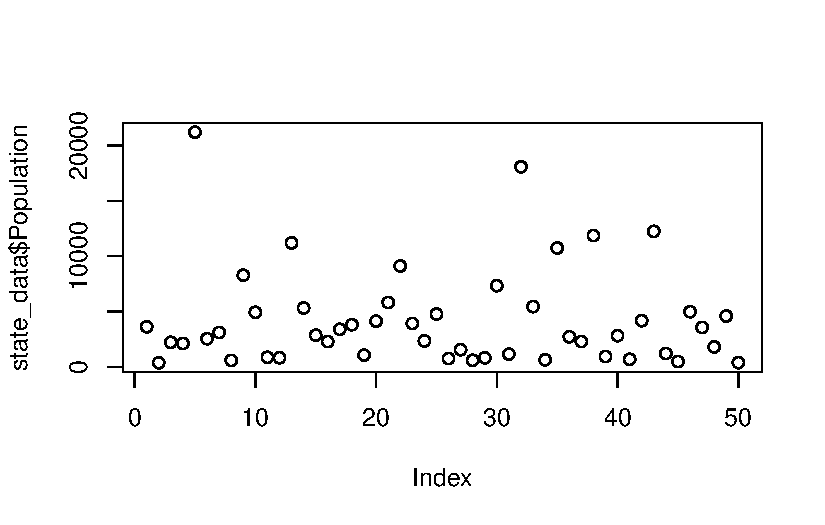
\includegraphics[keepaspectratio]{supervision_1_files/figure-pdf/unnamed-chunk-22-1.pdf}}

\textbf{Reflect:} What does this reveal about the distribution of state
populations?

\begin{center}\rule{0.5\linewidth}{0.5pt}\end{center}

\section{Part G --- Scatterplots}\label{part-g-scatterplots}

\begin{Shaded}
\begin{Highlighting}[]
\FunctionTok{plot}\NormalTok{(state\_data}\SpecialCharTok{$}\NormalTok{Income, state\_data}\SpecialCharTok{$}\NormalTok{Illiteracy)}
\end{Highlighting}
\end{Shaded}

\pandocbounded{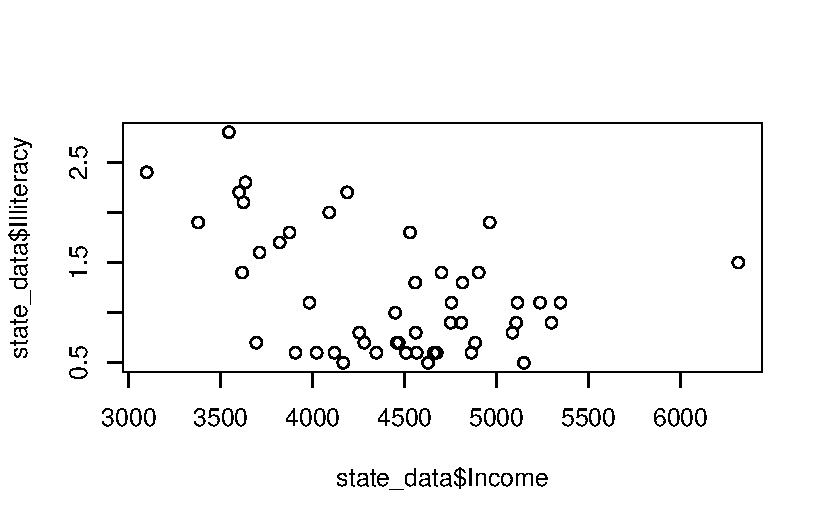
\includegraphics[keepaspectratio]{supervision_1_files/figure-pdf/unnamed-chunk-23-1.pdf}}

\textbf{Reflect:} Do states with higher income tend to have lower
illiteracy rates?

\begin{center}\rule{0.5\linewidth}{0.5pt}\end{center}

\section{Part H --- Entire dataset
plot}\label{part-h-entire-dataset-plot}

\begin{Shaded}
\begin{Highlighting}[]
\FunctionTok{plot}\NormalTok{(state\_data)}
\end{Highlighting}
\end{Shaded}

\pandocbounded{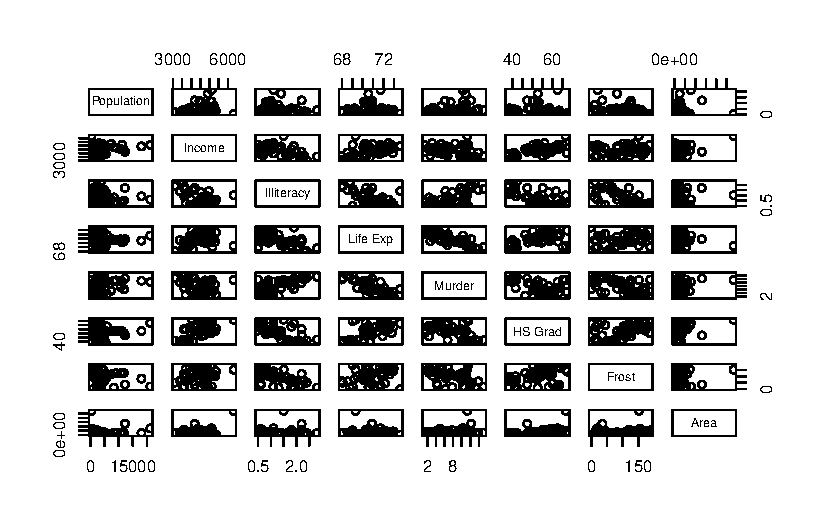
\includegraphics[keepaspectratio]{supervision_1_files/figure-pdf/unnamed-chunk-24-1.pdf}}

\textbf{Reflect:} Which pairs of socio-economic indicators appear
strongly related?

\begin{center}\rule{0.5\linewidth}{0.5pt}\end{center}

\section{Part I --- Points and lines}\label{part-i-points-and-lines}

\begin{Shaded}
\begin{Highlighting}[]
\FunctionTok{plot}\NormalTok{(state\_data}\SpecialCharTok{$}\StringTok{\textasciigrave{}}\AttributeTok{Life Exp}\StringTok{\textasciigrave{}}\NormalTok{, }\AttributeTok{type =} \StringTok{"b"}\NormalTok{)}
\end{Highlighting}
\end{Shaded}

\pandocbounded{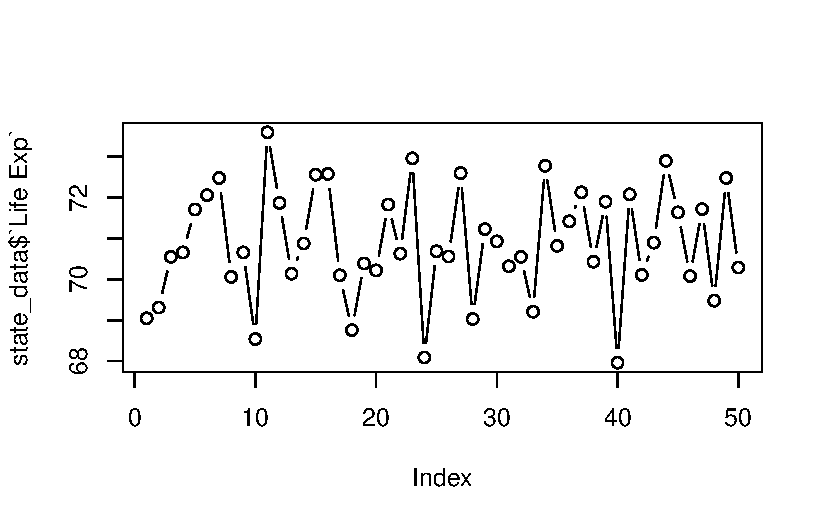
\includegraphics[keepaspectratio]{supervision_1_files/figure-pdf/unnamed-chunk-25-1.pdf}}

\begin{Shaded}
\begin{Highlighting}[]
\FunctionTok{plot}\NormalTok{(state\_data}\SpecialCharTok{$}\StringTok{\textasciigrave{}}\AttributeTok{Life Exp}\StringTok{\textasciigrave{}}\NormalTok{, }\AttributeTok{type =} \StringTok{"h"}\NormalTok{)}
\end{Highlighting}
\end{Shaded}

\pandocbounded{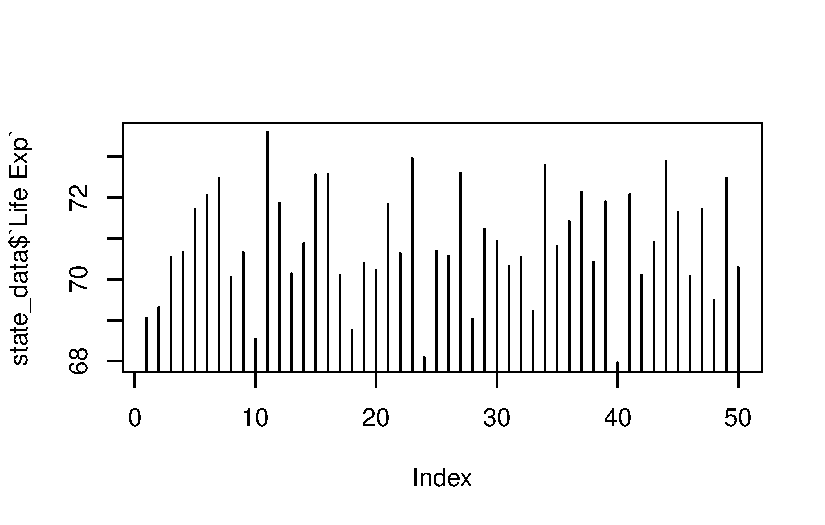
\includegraphics[keepaspectratio]{supervision_1_files/figure-pdf/unnamed-chunk-25-2.pdf}}

\textbf{Reflect:} Which representation communicates variation in life
expectancy more clearly?

\begin{center}\rule{0.5\linewidth}{0.5pt}\end{center}

\section{Part J --- Help}\label{part-j-help}

\begin{Shaded}
\begin{Highlighting}[]
\NormalTok{?plot}
\end{Highlighting}
\end{Shaded}

\begin{verbatim}
starting httpd help server ... done
\end{verbatim}

\textbf{Reflect:} Identify one new argument from the help page that
could improve your plot.

\begin{center}\rule{0.5\linewidth}{0.5pt}\end{center}

\section{Part K --- Labels and titles}\label{part-k-labels-and-titles}

\begin{Shaded}
\begin{Highlighting}[]
\FunctionTok{plot}\NormalTok{(state\_data}\SpecialCharTok{$}\NormalTok{Income,}
     \AttributeTok{xlab =} \StringTok{"State Index"}\NormalTok{,}
     \AttributeTok{ylab =} \StringTok{"Per Capita Income"}\NormalTok{,}
     \AttributeTok{main =} \StringTok{"Income levels across US states"}\NormalTok{,}
     \AttributeTok{col =} \StringTok{"blue"}\NormalTok{)}
\end{Highlighting}
\end{Shaded}

\pandocbounded{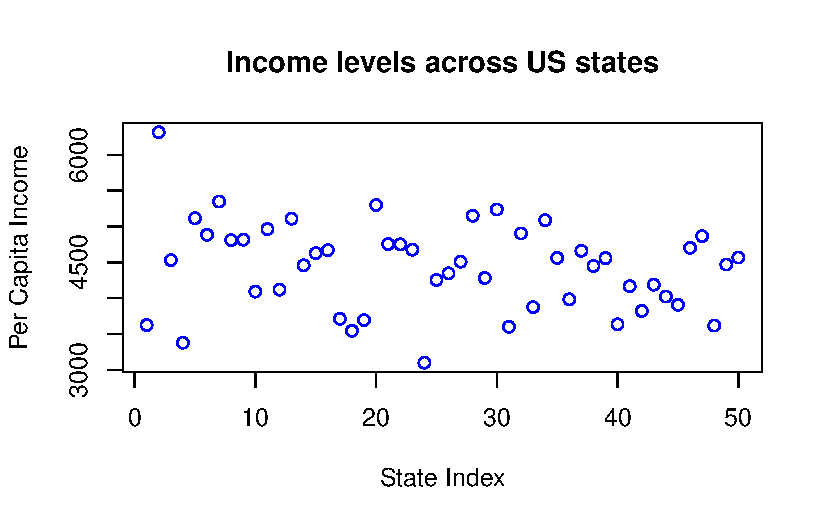
\includegraphics[keepaspectratio]{supervision_1_files/figure-pdf/unnamed-chunk-27-1.pdf}}

\textbf{Reflect:} Do the labels improve clarity? Suggest improvements if
needed.

\begin{center}\rule{0.5\linewidth}{0.5pt}\end{center}

\section{Part L --- Horizontal bar
plot}\label{part-l-horizontal-bar-plot}

\begin{Shaded}
\begin{Highlighting}[]
\FunctionTok{barplot}\NormalTok{(state\_data}\SpecialCharTok{$}\NormalTok{Murder,}
        \AttributeTok{main =} \StringTok{"Murder Rate by State"}\NormalTok{,}
        \AttributeTok{xlab =} \StringTok{"Murder arrests per 100,000"}\NormalTok{,}
        \AttributeTok{col =} \StringTok{"purple"}\NormalTok{,}
        \AttributeTok{horiz =} \ConstantTok{TRUE}\NormalTok{)}
\end{Highlighting}
\end{Shaded}

\pandocbounded{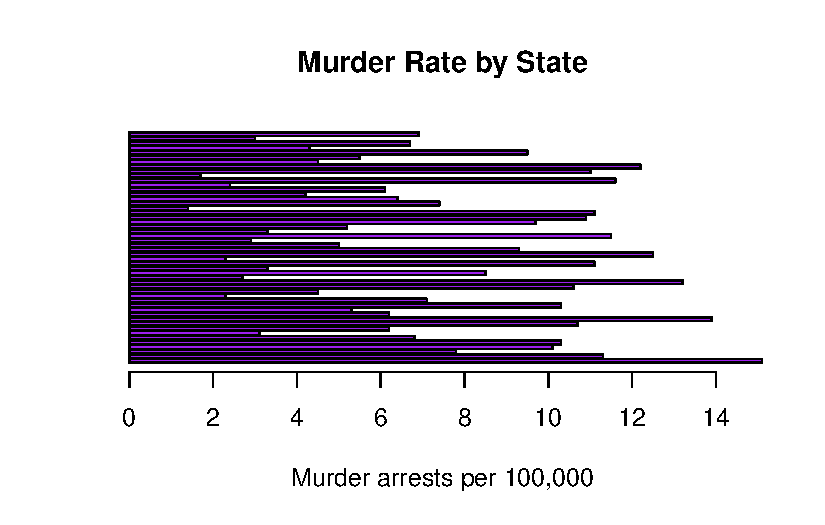
\includegraphics[keepaspectratio]{supervision_1_files/figure-pdf/unnamed-chunk-28-1.pdf}}

\textbf{Reflect:} Which states stand out with particularly high murder
rates?

\begin{center}\rule{0.5\linewidth}{0.5pt}\end{center}

\section{Part M --- Vertical bar plot}\label{part-m-vertical-bar-plot}

\begin{Shaded}
\begin{Highlighting}[]
\FunctionTok{barplot}\NormalTok{(state\_data}\SpecialCharTok{$}\NormalTok{Illiteracy,}
        \AttributeTok{main =} \StringTok{"Illiteracy Rate by State"}\NormalTok{,}
        \AttributeTok{xlab =} \StringTok{"\% Illiteracy"}\NormalTok{,}
        \AttributeTok{col =} \StringTok{"orange"}\NormalTok{,}
        \AttributeTok{horiz =} \ConstantTok{FALSE}\NormalTok{)}
\end{Highlighting}
\end{Shaded}

\pandocbounded{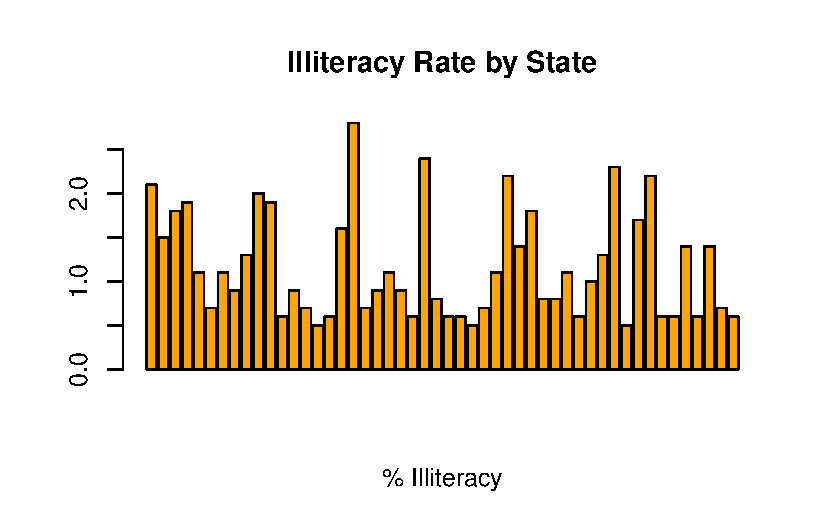
\includegraphics[keepaspectratio]{supervision_1_files/figure-pdf/unnamed-chunk-29-1.pdf}}

\textbf{Reflect:} How might this plot inform discussions on educational
policy?

\begin{center}\rule{0.5\linewidth}{0.5pt}\end{center}

\section{Part N --- Histograms}\label{part-n-histograms}

\begin{Shaded}
\begin{Highlighting}[]
\FunctionTok{hist}\NormalTok{(state\_data}\SpecialCharTok{$}\NormalTok{Income)}
\end{Highlighting}
\end{Shaded}

\pandocbounded{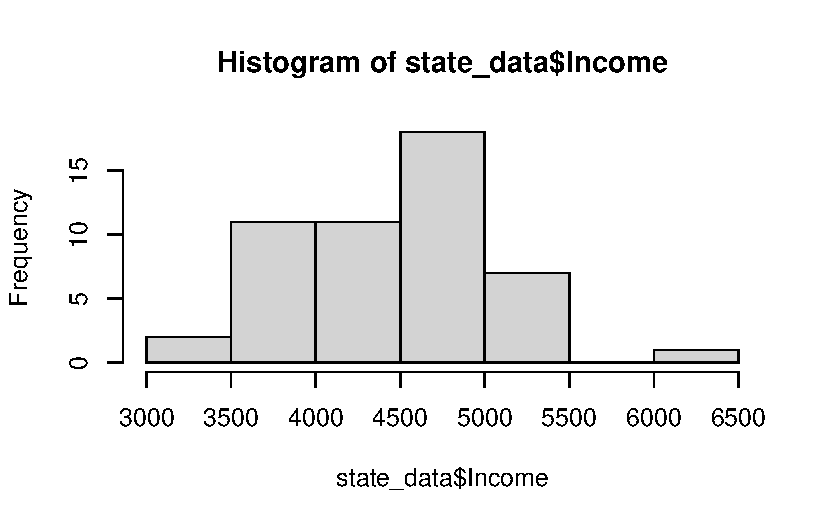
\includegraphics[keepaspectratio]{supervision_1_files/figure-pdf/unnamed-chunk-30-1.pdf}}

\begin{Shaded}
\begin{Highlighting}[]
\FunctionTok{hist}\NormalTok{(state\_data}\SpecialCharTok{$}\NormalTok{Income,}
     \AttributeTok{main =} \StringTok{"Distribution of State Incomes"}\NormalTok{,}
     \AttributeTok{xlab =} \StringTok{"Per Capita Income"}\NormalTok{,}
     \AttributeTok{col =} \StringTok{"green"}\NormalTok{)}
\end{Highlighting}
\end{Shaded}

\pandocbounded{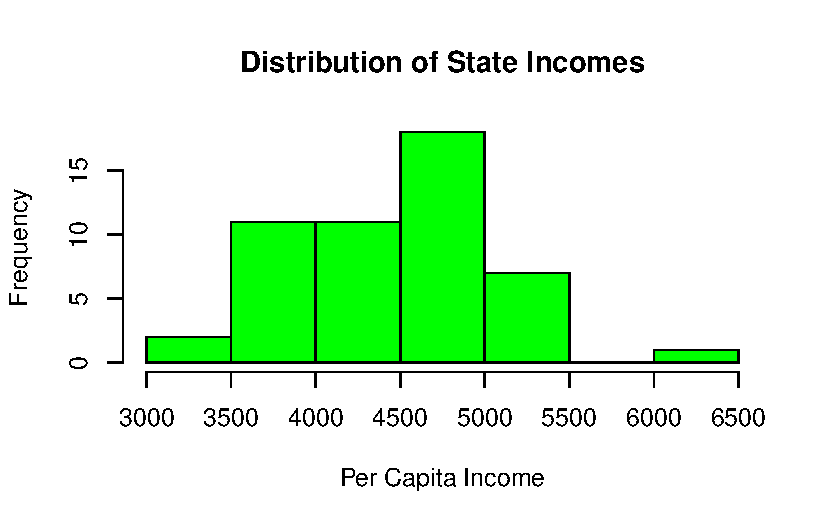
\includegraphics[keepaspectratio]{supervision_1_files/figure-pdf/unnamed-chunk-30-2.pdf}}

\textbf{Reflect:} Is the income distribution symmetric, skewed, or
multi-modal?

\begin{center}\rule{0.5\linewidth}{0.5pt}\end{center}

\section{Part O --- Boxplots}\label{part-o-boxplots}

\begin{Shaded}
\begin{Highlighting}[]
\FunctionTok{boxplot}\NormalTok{(state\_data}\SpecialCharTok{$}\StringTok{\textasciigrave{}}\AttributeTok{Life Exp}\StringTok{\textasciigrave{}}\NormalTok{)}
\end{Highlighting}
\end{Shaded}

\pandocbounded{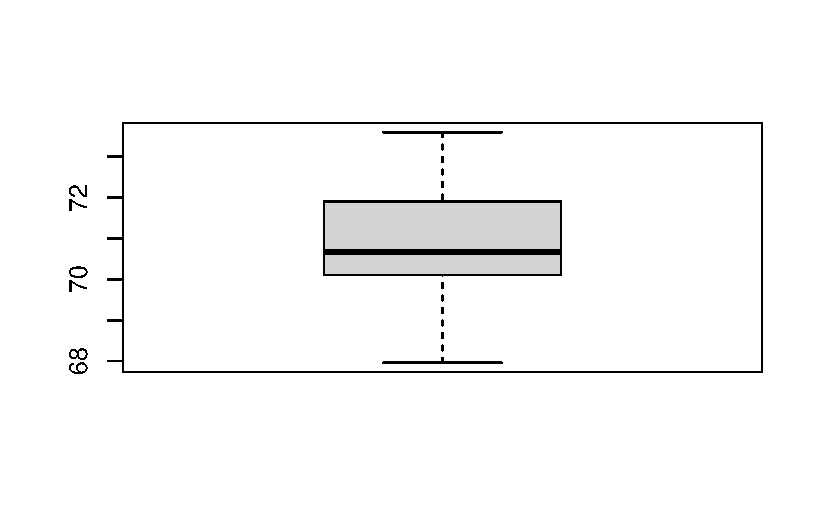
\includegraphics[keepaspectratio]{supervision_1_files/figure-pdf/unnamed-chunk-31-1.pdf}}

\textbf{Reflect:} What does the boxplot reveal about state-level life
expectancy?

\begin{center}\rule{0.5\linewidth}{0.5pt}\end{center}

\section{Part P --- Multiple boxplots}\label{part-p-multiple-boxplots}

\begin{Shaded}
\begin{Highlighting}[]
\FunctionTok{boxplot}\NormalTok{(state\_data[, }\FunctionTok{c}\NormalTok{(}\StringTok{"Population"}\NormalTok{, }\StringTok{"Income"}\NormalTok{, }\StringTok{"Illiteracy"}\NormalTok{, }\StringTok{"Life Exp"}\NormalTok{)],}
        \AttributeTok{main =} \StringTok{"Socio{-}economic Indicators across States"}\NormalTok{)}
\end{Highlighting}
\end{Shaded}

\pandocbounded{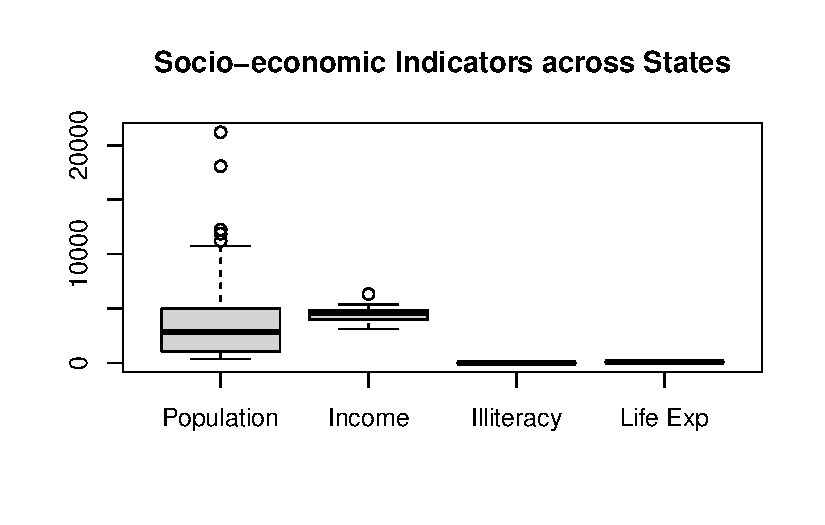
\includegraphics[keepaspectratio]{supervision_1_files/figure-pdf/unnamed-chunk-32-1.pdf}}

\textbf{Reflect:} Which variable shows the most variability? The least?

\begin{center}\rule{0.5\linewidth}{0.5pt}\end{center}

\section{Part Q --- Grid of charts}\label{part-q-grid-of-charts}

\begin{Shaded}
\begin{Highlighting}[]
\FunctionTok{par}\NormalTok{(}\AttributeTok{mfrow =} \FunctionTok{c}\NormalTok{(}\DecValTok{3}\NormalTok{,}\DecValTok{3}\NormalTok{), }\AttributeTok{mar =} \FunctionTok{c}\NormalTok{(}\DecValTok{2}\NormalTok{,}\DecValTok{5}\NormalTok{,}\DecValTok{2}\NormalTok{,}\DecValTok{1}\NormalTok{), }\AttributeTok{las =} \DecValTok{1}\NormalTok{, }\AttributeTok{bty =} \StringTok{"n"}\NormalTok{)}

\FunctionTok{plot}\NormalTok{(state\_data}\SpecialCharTok{$}\NormalTok{Population)}
\FunctionTok{plot}\NormalTok{(state\_data}\SpecialCharTok{$}\NormalTok{Income, state\_data}\SpecialCharTok{$}\NormalTok{Illiteracy)}
\FunctionTok{plot}\NormalTok{(state\_data}\SpecialCharTok{$}\StringTok{\textasciigrave{}}\AttributeTok{Life Exp}\StringTok{\textasciigrave{}}\NormalTok{, }\AttributeTok{type =} \StringTok{"c"}\NormalTok{)}
\FunctionTok{plot}\NormalTok{(state\_data}\SpecialCharTok{$}\StringTok{\textasciigrave{}}\AttributeTok{Life Exp}\StringTok{\textasciigrave{}}\NormalTok{, }\AttributeTok{type =} \StringTok{"s"}\NormalTok{)}
\FunctionTok{plot}\NormalTok{(state\_data}\SpecialCharTok{$}\StringTok{\textasciigrave{}}\AttributeTok{Life Exp}\StringTok{\textasciigrave{}}\NormalTok{, }\AttributeTok{type =} \StringTok{"h"}\NormalTok{)}
\FunctionTok{barplot}\NormalTok{(state\_data}\SpecialCharTok{$}\NormalTok{Income, }\AttributeTok{main =} \StringTok{"Income levels"}\NormalTok{, }\AttributeTok{col =} \StringTok{"blue"}\NormalTok{, }\AttributeTok{horiz =} \ConstantTok{TRUE}\NormalTok{)}
\FunctionTok{hist}\NormalTok{(state\_data}\SpecialCharTok{$}\NormalTok{Murder)}
\FunctionTok{boxplot}\NormalTok{(state\_data}\SpecialCharTok{$}\StringTok{\textasciigrave{}}\AttributeTok{HS Grad}\StringTok{\textasciigrave{}}\NormalTok{)}
\FunctionTok{boxplot}\NormalTok{(state\_data[, }\FunctionTok{c}\NormalTok{(}\StringTok{"Population"}\NormalTok{, }\StringTok{"Income"}\NormalTok{, }\StringTok{"Illiteracy"}\NormalTok{, }\StringTok{"Life Exp"}\NormalTok{)],}
        \AttributeTok{main =} \StringTok{"Multiple Box plots"}\NormalTok{)}
\end{Highlighting}
\end{Shaded}

\pandocbounded{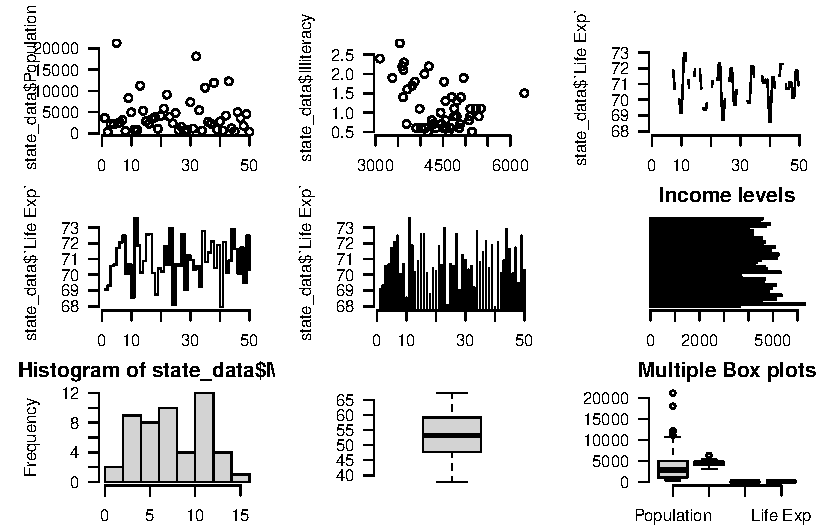
\includegraphics[keepaspectratio]{supervision_1_files/figure-pdf/unnamed-chunk-33-1.pdf}}

\textbf{Reflect:} Which plots are most useful for policy discussions?
Which are least useful?

\begin{center}\rule{0.5\linewidth}{0.5pt}\end{center}

\section{Best practices}\label{best-practices-3}

\begin{itemize}
\tightlist
\item
  Always check the structure of socio-economic data before plotting.
\item
  Match plot type to variable type.
\item
  Add descriptive titles and labels.
\item
  Avoid misleading graphics (bar plots for continuous data should be
  used cautiously).
\item
  Visualise relationships before modelling.
\end{itemize}

\begin{center}\rule{0.5\linewidth}{0.5pt}\end{center}

\section{Further visualisation
packages}\label{further-visualisation-packages}

\begin{itemize}
\tightlist
\item
  \textbf{lattice}: kernel density plots
\item
  \textbf{ggplot2}: flexible grammar of graphics
\item
  \textbf{plotly}: interactive plots
\item
  \textbf{maps}: plot country maps
\end{itemize}

More resources:
\href{https://towardsdatascience.com/a-guide-to-data-visualisation-in-r-for-beginners-ef6d41a34174}{towardsdatascience.com
article}

\begin{center}\rule{0.5\linewidth}{0.5pt}\end{center}

\section{Suggested Answers to Reflection
Questions}\label{suggested-answers-to-reflection-questions-1}

\begin{itemize}
\tightlist
\item
  \textbf{Part A:} Variables include Population, Income, Illiteracy,
  Life Expectancy, Murder rate, HS graduation, Frost, and Area. Most
  relate directly to planning and socio-economic development.
\item
  \textbf{Part B:} 50 rows (states) and 8 columns. All variables are
  numeric.
\item
  \textbf{Part C:} States differ widely in population and area; later
  rows (western states) often have larger land areas.
\item
  \textbf{Part D:} Population and Area show the widest spread.
\item
  \textbf{Part F:} Populations vary dramatically; California, New York,
  Texas are clear outliers.
\item
  \textbf{Part G:} Clear negative relationship: higher income states
  tend to have lower illiteracy.
\item
  \textbf{Part H:} Income vs Illiteracy, Life Expectancy vs Murder, and
  Population vs Area show strong patterns.
\item
  \textbf{Part I:} Type ``b'' (points and lines) is clearer for showing
  gradual variation than type ``h'' (histogram-like lines).
\item
  \textbf{Part J:} Useful arguments include \texttt{pch} (point type)
  and \texttt{col} (colour).
\item
  \textbf{Part K:} Labels help; better axis labels might specify units
  (e.g., dollars, years).
\item
  \textbf{Part L:} Southern states often stand out with higher murder
  rates.
\item
  \textbf{Part M:} Highlights disparities in illiteracy across regions;
  relevant to education policy.
\item
  \textbf{Part N:} Income is slightly right-skewed; most states cluster
  around the middle with a few richer outliers.
\item
  \textbf{Part O:} Median life expectancy around 70 years; some outliers
  with lower values.
\item
  \textbf{Part P:} Population and Area show the most variability; Life
  Expectancy the least.
\item
  \textbf{Part Q:} Scatterplot of Income vs Illiteracy and histogram of
  Murder are most useful for policy; line-type plots of Life Expectancy
  less so.
\end{itemize}

\begin{center}\rule{0.5\linewidth}{0.5pt}\end{center}

\section{Suggested Answers to Reflection
Questions}\label{suggested-answers-to-reflection-questions-2}

\begin{quote}
These are concise, indicative answers. Local results may vary slightly
depending on plotting parameters and ordering.
\end{quote}

\subsection{Part A --- Load dataset}\label{part-a-load-dataset-1}

\begin{itemize}
\tightlist
\item
  Variables in \texttt{state.x77}: \texttt{Population} (thousands),
  \texttt{Income} (per-capita, USD), \texttt{Illiteracy} (\% age ≥25
  illiterate), \texttt{Life.Exp} (years), \texttt{Murder} (per 100,000),
  \texttt{HS.Grad} (\% high-school graduates), \texttt{Frost} (mean days
  ≤ 0°C), \texttt{Area} (square miles).\\
\item
  Planning relevance: population size/density, income, education, crime,
  longevity connect to regional disparities and regeneration priorities.
\end{itemize}

\subsection{Part B --- Data
exploration}\label{part-b-data-exploration-1}

\begin{itemize}
\tightlist
\item
  Dimensions: \textbf{50 rows × 8 columns}.\\
\item
  All columns are numeric/continuous; state names are row names
  (categorical identifier).
\end{itemize}

\subsection{Part C --- Head/Tail}\label{part-c-headtail}

\begin{itemize}
\tightlist
\item
  Early vs late rows simply reflect alphabetical state ordering; no time
  component. Values vary widely (e.g., \texttt{Area},
  \texttt{Population}).
\end{itemize}

\subsection{Part D --- Descriptive
statistics}\label{part-d-descriptive-statistics-1}

\begin{itemize}
\tightlist
\item
  Widest spreads typically in \texttt{Area} and \texttt{Population}
  (large range, right-skew).\\
\item
  \texttt{Murder} and \texttt{Illiteracy} show noticeable skew and
  outliers.
\end{itemize}

\subsection{Part E --- Graphics help}\label{part-e-graphics-help}

\begin{itemize}
\tightlist
\item
  Useful base functions: \texttt{pairs()}, \texttt{boxplot()},
  \texttt{hist()}, \texttt{barplot()}, \texttt{stripchart()},
  \texttt{dotchart()}, \texttt{qqnorm()}/\texttt{qqline()}.
\end{itemize}

\subsection{Part F --- Single column plot
(Population)}\label{part-f-single-column-plot-population}

\begin{itemize}
\tightlist
\item
  Strong right-skew: a few very populous states (CA, NY, TX) vs many
  smaller states. Outliers at the high end.
\end{itemize}

\subsection{Part G --- Scatter (Income vs
Illiteracy)}\label{part-g-scatter-income-vs-illiteracy}

\begin{itemize}
\tightlist
\item
  Clear \textbf{negative} association: higher income correlates with
  lower illiteracy.\\
\item
  Some states deviate from the trend but pattern holds overall.
\end{itemize}

\subsection{\texorpdfstring{Part H --- \texttt{pairs()} of entire
dataset}{Part H --- pairs() of entire dataset}}\label{part-h-pairs-of-entire-dataset}

\begin{itemize}
\tightlist
\item
  Notable patterns often seen:

  \begin{itemize}
  \tightlist
  \item
    \texttt{Income} ↑ with \texttt{HS.Grad} and \texttt{Life.Exp}.\\
  \item
    \texttt{Murder} tends to be higher where \texttt{Illiteracy} is
    higher and \texttt{HS.Grad} is lower.\\
  \item
    \texttt{Area} weakly related to socio-economic outcomes (size ≠
    prosperity).
  \end{itemize}
\end{itemize}

\subsection{Part I --- Types ``b'' vs ``h''
(Life.Exp)}\label{part-i-types-b-vs-h-life.exp}

\begin{itemize}
\tightlist
\item
  \texttt{type="b"} conveys point-to-point variability;
  \texttt{type="h"} emphasizes magnitudes from baseline.\\
\item
  For life expectancy, \texttt{"b"} is generally clearer.
\end{itemize}

\subsection{Part J --- Help}\label{part-j-help-1}

\begin{itemize}
\tightlist
\item
  Examples of useful args: \texttt{pch} (point symbol), \texttt{cex}
  (size), \texttt{col} (colour), \texttt{xlim}/\texttt{ylim} (ranges),
  \texttt{main}/\texttt{sub} (titles/subtitles).
\end{itemize}

\subsection{Part K --- Labels and titles
(Income)}\label{part-k-labels-and-titles-income}

\begin{itemize}
\tightlist
\item
  Better labels: x = ``State (index)'', y = ``Per-capita income (USD)'',
  title = ``Per-capita income by state''.\\
\item
  Colour is decorative here unless encoding a grouping.
\end{itemize}

\subsection{Part L --- Horizontal bar plot
(Murder)}\label{part-l-horizontal-bar-plot-murder}

\begin{itemize}
\tightlist
\item
  States with higher values stand out (exact names depend on ordering).
  For rigorous identification, sort with \texttt{order()} or use a
  dotchart.
\end{itemize}

\subsection{Part M --- Vertical bar plot
(Illiteracy)}\label{part-m-vertical-bar-plot-illiteracy}

\begin{itemize}
\tightlist
\item
  Helps compare education disparities. Policy angle: target states with
  highest illiteracy for adult education and schooling investment.
\end{itemize}

\subsection{Part N --- Histogram
(Income)}\label{part-n-histogram-income}

\begin{itemize}
\tightlist
\item
  Typically unimodal, mild right-skew. Most states cluster around
  mid-income; a few richer states in the right tail. Bin choice affects
  apparent shape.
\end{itemize}

\subsection{Part O --- Boxplot
(Life.Exp)}\label{part-o-boxplot-life.exp}

\begin{itemize}
\tightlist
\item
  Median around \textasciitilde70 years, relatively tight IQR; lower
  outliers indicate states with comparatively worse health outcomes.
\end{itemize}

\subsection{Part P --- Multiple
boxplots}\label{part-p-multiple-boxplots-1}

\begin{itemize}
\tightlist
\item
  \texttt{Population} shows largest spread; \texttt{Life.Exp} the
  tightest. Outliers are more common in \texttt{Murder} and
  \texttt{Illiteracy}.
\end{itemize}

\subsection{Part Q --- Grid of charts}\label{part-q-grid-of-charts-1}

\begin{itemize}
\tightlist
\item
  Most informative: scatterplots for relationships (e.g.,
  \texttt{Income} vs \texttt{Illiteracy}), and boxplots/histograms for
  distributions.\\
\item
  Least informative: unsorted barplots of continuous variables.
\end{itemize}

\subsection{Best practices ---
summaries}\label{best-practices-summaries}

\begin{itemize}
\tightlist
\item
  Inspect structure first; match plot to variable type; label clearly;
  avoid misleading encodings; explore visually before modelling.
\end{itemize}

\emph{End of Lab 4}

\bookmarksetup{startatroot}

\chapter{Lab 5 --- Using GitHub Copilot in
RStudio}\label{lab-5-using-github-copilot-in-rstudio}

\section{Goal}\label{goal}

Learn to use GitHub Copilot inside RStudio to speed up routine coding,
while staying in control of quality, privacy, and reproducibility.

\begin{center}\rule{0.5\linewidth}{0.5pt}\end{center}

\section{Learning outcomes}\label{learning-outcomes-4}

By the end you will be able to: 1. Enable and sign into GitHub Copilot
in RStudio. 2. Accept, reject, or modify Copilot autocomplete
suggestions effectively. 3. Use comment-first prompting to steer
suggestions. 4. Diagnose and fix typical Copilot mistakes (wrong column
names, redundant args, etc.). 5. Apply safe-use practices (privacy,
determinism, avoiding ``vibe coding'').

\begin{center}\rule{0.5\linewidth}{0.5pt}\end{center}

\section{Prerequisites}\label{prerequisites-4}

\begin{itemize}
\tightlist
\item
  R (≥ 4.3 recommended) and RStudio (a recent version with Copilot
  support).
\item
  A GitHub account with Copilot access (student/educator plans are
  available).
\item
  Packages: \texttt{tidyverse}, \texttt{palmerpenguins},
  \texttt{readxl}, \texttt{ggplot2}.
\end{itemize}

\begin{Shaded}
\begin{Highlighting}[]
\FunctionTok{install.packages}\NormalTok{(}\FunctionTok{c}\NormalTok{(}\StringTok{"tidyverse"}\NormalTok{, }\StringTok{"palmerpenguins"}\NormalTok{, }\StringTok{"readxl"}\NormalTok{, }\StringTok{"ggplot2"}\NormalTok{))}
\end{Highlighting}
\end{Shaded}

\begin{quote}
Note: Column names for the \texttt{penguins} dataset may differ
depending on source. Treat this as a feature to practice Copilot-aware
debugging.
\end{quote}

\begin{center}\rule{0.5\linewidth}{0.5pt}\end{center}

\section{Part A --- Set up Copilot in RStudio (10--15
min)}\label{part-a-set-up-copilot-in-rstudio-1015-min}

\begin{enumerate}
\def\labelenumi{\arabic{enumi}.}
\tightlist
\item
  Open RStudio → Tools → Global Options → Copilot.
\item
  Enable GitHub Copilot and sign in with GitHub.
\item
  Create a new R Script (\texttt{File\ →\ New\ File\ →\ R\ Script}).
\item
  Type some characters to see ghost text suggestions.

  \begin{itemize}
  \tightlist
  \item
    Tab to accept, Esc to dismiss, or keep typing to ignore.
  \end{itemize}
\end{enumerate}

\subsection{Reflection A}\label{reflection-a}

Explain in one sentence the difference between ghost text and code
you've actually inserted.

\begin{center}\rule{0.5\linewidth}{0.5pt}\end{center}

\section{Part B --- First suggestions with ggplot2 (20
min)}\label{part-b-first-suggestions-with-ggplot2-20-min}

We'll use \texttt{penguins} to practice.

\begin{enumerate}
\def\labelenumi{\arabic{enumi}.}
\tightlist
\item
  Add a guiding comment:
\end{enumerate}

\begin{Shaded}
\begin{Highlighting}[]
\CommentTok{\# Task: scatter plot of bill length (x) vs body mass (y), colour by species}
\end{Highlighting}
\end{Shaded}

\begin{enumerate}
\def\labelenumi{\arabic{enumi}.}
\setcounter{enumi}{1}
\tightlist
\item
  Start a plot:
\end{enumerate}

\begin{Shaded}
\begin{Highlighting}[]
\FunctionTok{library}\NormalTok{(ggplot2)}
\CommentTok{\# library(palmerpenguins)}
\CommentTok{\# penguins \textless{}{-} palmerpenguins::penguins}

\NormalTok{p }\OtherTok{\textless{}{-}} \FunctionTok{ggplot}\NormalTok{(penguins, }\FunctionTok{aes}\NormalTok{(}\AttributeTok{x =}\NormalTok{ bill\_length\_mm, }\AttributeTok{y =}\NormalTok{ body\_mass\_g, }\AttributeTok{colour =}\NormalTok{ species)) }\SpecialCharTok{+}
  \FunctionTok{geom\_point}\NormalTok{()}
\end{Highlighting}
\end{Shaded}

\begin{enumerate}
\def\labelenumi{\arabic{enumi}.}
\setcounter{enumi}{2}
\tightlist
\item
  Run and, if errors occur, inspect:
\end{enumerate}

\begin{Shaded}
\begin{Highlighting}[]
\FunctionTok{glimpse}\NormalTok{(penguins)}
\FunctionTok{names}\NormalTok{(penguins)}
\end{Highlighting}
\end{Shaded}

\begin{enumerate}
\def\labelenumi{\arabic{enumi}.}
\setcounter{enumi}{3}
\tightlist
\item
  Fix names if needed (\texttt{bill\_length\_mm} → \texttt{bill\_len}).
\end{enumerate}

\subsection{Mini-exercises}\label{mini-exercises}

\begin{itemize}
\tightlist
\item
  Add title, caption, and axis labels:
\end{itemize}

\begin{Shaded}
\begin{Highlighting}[]
\CommentTok{\# Add a title, caption, and nicer axis labels}
\end{Highlighting}
\end{Shaded}

\begin{itemize}
\tightlist
\item
  Add smoother:
\end{itemize}

\begin{Shaded}
\begin{Highlighting}[]
\CommentTok{\# Add a loess smoother without confidence band}
\end{Highlighting}
\end{Shaded}

\subsection{Reflection B}\label{reflection-b}

When is Copilot faster? When slower?

\begin{center}\rule{0.5\linewidth}{0.5pt}\end{center}

\section{Part C --- Comment-first prompting for histograms (15
min)}\label{part-c-comment-first-prompting-for-histograms-15-min}

\begin{enumerate}
\def\labelenumi{\arabic{enumi}.}
\tightlist
\item
  Add a guiding comment:
\end{enumerate}

\begin{Shaded}
\begin{Highlighting}[]
\CommentTok{\# Histogram of body mass by species, overlapping with transparency and an accessible palette}
\end{Highlighting}
\end{Shaded}

\begin{enumerate}
\def\labelenumi{\arabic{enumi}.}
\setcounter{enumi}{1}
\tightlist
\item
  Inspect Copilot's suggestion, remove redundant arguments, and adjust
  to:
\end{enumerate}

\begin{Shaded}
\begin{Highlighting}[]
\FunctionTok{geom\_histogram}\NormalTok{(}\AttributeTok{position =} \StringTok{"identity"}\NormalTok{, }\AttributeTok{alpha =} \FloatTok{0.5}\NormalTok{)}
\end{Highlighting}
\end{Shaded}

\begin{enumerate}
\def\labelenumi{\arabic{enumi}.}
\setcounter{enumi}{2}
\tightlist
\item
  Commit the cleaned version.
\end{enumerate}

\subsection{Reflection C}\label{reflection-c}

Replace colour with \texttt{fill}, adjust legend, apply minimal theme.

\begin{center}\rule{0.5\linewidth}{0.5pt}\end{center}

\section{Part D --- Loading local data safely (10--15
min)}\label{part-d-loading-local-data-safely-1015-min}

Copilot does not know your file system.

\begin{enumerate}
\def\labelenumi{\arabic{enumi}.}
\tightlist
\item
  Save \texttt{Scooby.xlsx} in a \texttt{data/} folder.
\item
  Load explicitly:
\end{enumerate}

\begin{Shaded}
\begin{Highlighting}[]
\FunctionTok{library}\NormalTok{(readxl)}
\NormalTok{scooby }\OtherTok{\textless{}{-}} \FunctionTok{read\_xlsx}\NormalTok{(}\StringTok{"data/Scooby.xlsx"}\NormalTok{)}
\end{Highlighting}
\end{Shaded}

\begin{enumerate}
\def\labelenumi{\arabic{enumi}.}
\setcounter{enumi}{2}
\tightlist
\item
  Add prompt:
\end{enumerate}

\begin{Shaded}
\begin{Highlighting}[]
\CommentTok{\# Quick EDA: glimpse, summary, and count episodes by network}
\end{Highlighting}
\end{Shaded}

\begin{enumerate}
\def\labelenumi{\arabic{enumi}.}
\setcounter{enumi}{3}
\tightlist
\item
  Edit Copilot's code before running.
\end{enumerate}

\subsection{Reflection D}\label{reflection-d}

Why be explicit with data loading and library imports?

\begin{center}\rule{0.5\linewidth}{0.5pt}\end{center}

\section{Part E --- Boxplots (15 min)}\label{part-e-boxplots-15-min}

Visualise IMDb ratings by network.

\begin{enumerate}
\def\labelenumi{\arabic{enumi}.}
\tightlist
\item
  Prompt:
\end{enumerate}

\begin{Shaded}
\begin{Highlighting}[]
\CommentTok{\# Boxplot of IMDb (y) by network (x); tilt x labels; use fill instead of colour}
\end{Highlighting}
\end{Shaded}

\begin{enumerate}
\def\labelenumi{\arabic{enumi}.}
\setcounter{enumi}{1}
\tightlist
\item
  Edit column names if needed.
\item
  Add improvements:
\end{enumerate}

\begin{Shaded}
\begin{Highlighting}[]
\CommentTok{\# Make it horizontal, tidy legend, and add labs}
\end{Highlighting}
\end{Shaded}

\subsection{Extension E}\label{extension-e}

Order networks by median rating.

\begin{center}\rule{0.5\linewidth}{0.5pt}\end{center}

\section{Part F --- Best practices}\label{part-f-best-practices}

\begin{itemize}
\tightlist
\item
  Privacy: Never expose credentials/confidential data.
\item
  Non-determinism: Review suggestions before accepting.
\item
  No vibe coding: Don't accept what you don't understand.
\item
  Context helps: Use clean code and comments.
\item
  Reproducibility: Remove redundant args, consider \texttt{renv}.
\end{itemize}

\begin{Shaded}
\begin{Highlighting}[]
\FunctionTok{install.packages}\NormalTok{(}\StringTok{"renv"}\NormalTok{)}
\NormalTok{renv}\SpecialCharTok{::}\FunctionTok{init}\NormalTok{()}
\end{Highlighting}
\end{Shaded}

\begin{center}\rule{0.5\linewidth}{0.5pt}\end{center}

\section{Part G --- Check-off \&
submission}\label{part-g-check-off-submission}

\begin{itemize}
\tightlist
\item[$\square$]
  Copilot enabled and signed in.
\item[$\square$]
  One scatter plot (corrected column names).
\item[$\square$]
  One histogram (transparency + accessible palette).
\item[$\square$]
  One boxplot (labels/theme improved).
\item[$\square$]
  Reflection paragraph on Copilot.
\end{itemize}

Export script or Quarto doc → submit.

\begin{center}\rule{0.5\linewidth}{0.5pt}\end{center}

\section{TA rubric}\label{ta-rubric}

\begin{itemize}
\tightlist
\item
  Setup (10\%): Copilot enabled; script compiles.
\item
  Code quality (40\%): Reviewed/edited suggestions; correct names.
\item
  Visuals (30\%): Clear labels, sensible themes.
\item
  Reflection (20\%): Insightful, acknowledges limits.
\end{itemize}

\begin{center}\rule{0.5\linewidth}{0.5pt}\end{center}

\section{Troubleshooting}\label{troubleshooting}

\begin{itemize}
\tightlist
\item
  Suggestions not appearing? Check Global Options → Copilot.
\item
  Wrong dataset/columns? Run \texttt{names()}/\texttt{glimpse()}.
\item
  Overconfident code? Scale back, test small steps.
\end{itemize}

\begin{center}\rule{0.5\linewidth}{0.5pt}\end{center}

\section{Further practice}\label{further-practice}

\begin{itemize}
\tightlist
\item
  Rewrite prompts as comments for grouped summaries, joins, faceted
  plots.
\item
  Compare Copilot vs manual solutions.
\item
  Try Quarto docs where each chunk begins with a comment.
\end{itemize}

\begin{center}\rule{0.5\linewidth}{0.5pt}\end{center}

End of lab




\end{document}
